\documentclass{article}
\usepackage{graphicx} % Required for inserting images
\usepackage[a4paper, total={6in, 8in}]{geometry}
\usepackage{titlesec}
\usepackage{amssymb}
\usepackage{setspace}
\usepackage{amsmath}
\usepackage{amsthm}
\usepackage[
   backend=biber,
   sorting=nyt,
   citestyle=alphabetic-verb,
   bibstyle=alphabetic,
]{biblatex}
\usepackage{minted}
\usepackage[T1]{fontenc}
\usepackage[sfdefault]{biolinum}
\usepackage{hyperref}
\usepackage{unicode-math}

\addbibresource{bibliography.bib}

\newtheorem{definition}{Définition}
\newtheorem{property}{Propriété}
\newtheorem{proposition}{Proposition}
\newtheorem{lemma}{Lemme}
\newtheorem{theorem}{Théorème}
\newtheorem{corollary}{Corollaire}
\theoremstyle{remark}
\newtheorem*{remark}{Remarque}
\theoremstyle{remark}
\newtheorem*{notation}{Notation}

\newcommand{\preb}[1]{{}^\bullet #1}
\newcommand{\postb}[1]{#1^\bullet}
\newcommand{\reach}[3][]{\mathcal{R}^{#1}(\mathcal{#2}, #3)}
\newcommand{\creach}[3][]{\mathbb{Q}\reach[#1]{#2}{#3}}
\newcommand{\reaches}[1][]{\xrightarrow{#1}}
\newcommand{\reachess}{\reaches^*}
\newcommand{\creaches}[1][]{\reaches[#1]_{\mathbb{Q}}}
\newcommand{\creachess}{\creaches^*}
\newcommand{\natinduction}[5]{
    Posons $\mathcal{#1}(n)$ la propriété \[#3.\]
    Montrons $\mathcal{#1}(n)$ par récurrence sur tout $n \in #2$.\\
    \textit{Cas de base.} #4\\
    \textit{Cas héréditaire.} Supposons $\mathcal{#1}(n)$ pour un certain $n \in #2$. #5
}
\newcommand{\induction}[3]{
    \textit{Cas de base.} #2\\
    \textit{Cas héréditaire.} Supposons la propriété vraie pour un certain $n \in #1$. #3
}
\newcommand{\restrict}[2]{#1_{|_{#2}}}
\newcommand{\extend}[1][\cdot]{\langle #1 \rangle}
\newcommand{\coextend}[1][\cdot]{\extend[#1]_+}
\newcommand{\rcoextend}[1][\cdot]{\coextend[#1]^{-1}}
\newcommand{\prototype}[3]{#1 : #2 \rightarrow #3}
\newcommand{\function}[5]{
    \begin{tabular}{r c c c}
         $#1 :$ & $#2$ & $\rightarrow$ & $#3$ \\
                & $#4$ &   $\mapsto$   & $#5$
    \end{tabular}
}
\newcommand{\indicator}{\mathbb{1}}
\newcommand{\runs}[2][]{\mathcal{E}^{#1}(\mathcal{#2})}
\newcommand{\execpath}[1]{\langle \! \langle #1 \rangle \! \rangle}

\renewcommand*\contentsname{Table des matières}
\renewcommand{\abstractname}{Résumé}
\renewcommand{\proofname}{Démonstration}
\renewcommand{\labelenumi}{(\roman{enumi})}

\setlength{\parskip}{10pt}
\setmathfont{NewCMMath-Book}

\title{Étude des réseaux de Petri continus\\et extensions structurelles}
\author{Arthur Barbera}
\date{Mai 2026}

\begin{document}

\maketitle

\begin{abstract}
    Nous reprenons dans ce document les extensions d'arcs implémentés dans les réseaux de Petri discrets permettant d'améliorer leur expressivité. Nous utilisons la sémantique des réseaux continus qui permet d'approximer le comportement des réseaux discrets dans le but d'établir de nouveaux résultats au problème d'accessibilité. Ce dernier est indécidable dans les réseaux classiques en la présence de chacun des arcs inhibiteur, de reset et de transfert.
    
    En partant de la motivation selon laquelle les réseaux continus ont permis de faire passer le problème d'accessibilité d'$\mathrm{Ackermann-complete}$ dans les réseaux classiques à $\mathrm{P}$ dans la variante continue, nous faisons de même en définissant une sémantique adaptée des arcs étendus dans les réseaux de Petri continus étendus.

    Nous créons tout d'abord un lien entre le problème d'accessibilité des réseaux continus à arcs inhibiteurs adoptant une certaine structure et le problème de l'arrêt d'une machine de Minsky ; puis, nous nous appuyons sur un isomorphisme entre les marquages des réseaux à arcs inhibiteurs et à arcs de reset afin de prouver l'équivalence de leurs fonctionnements respectifs.

    C'est ainsi que nous prouvons que le caractère indécidable du problème d'accessibilité persiste dans les réseaux de Petri continus étendus par des arcs inhibiteurs et de reset.
\end{abstract}

\newpage

\tableofcontents

\newpage

\addcontentsline{toc}{section}{Introduction}
\section*{Introduction}

\textbf{À rédiger.}

% De nombreux articles scientifiques tentent de résoudre ou d'améliorer la complexité du problème d'accessibilité des réseaux de Petri. Celui-ci, qualifié d'Ackermann-complet, se concentre sur la décidabilité du caractère accessible d'un marquage au sein du réseau en partant d'un marquage initial et en tirant de façon successive un ensemble de transitions. Il existe de plus une dérivée des réseaux de Petri permettant d'augmenter leur expressivité. Ceux-ci, sobrement nommés réseaux étendus, adoptent de nouvelles structures d'arcs reposant sur des sémantiques distinctes : lecture, test à 0, reset et transfert de jetons. Dans les trois derniers cas, il est prouvé que l'accessibilité devient indécidable. Afin d'améliorer la complexité de l'accessibilité des réseaux de Petri, une variante continue a été établie et permet d'approximer le comportement de leurs pairs discrets. Ce projet porte ses fruits car il transfère le problème dans la classe $\mathrm{P}$.

% Dans ce document, nous nous intéressons premièrement aux réseaux de Petri discrets classiques. Ce modèle de calcul est utilisé dans divers secteurs de l'informatique : programmation concurrentielle, automatisme, etc. Nous allons définir formellement les concepts clés, énoncer des lemmes et propriétés s'y rattachant puis voir certains résultats aux problèmes les plus importants. Ce type de réseau a vu son expressivité être augmentée via des extensions au niveau des arcs. En effet, certains d'entre eux augmentent l'expressivité du réseau, au détriment de la décidabilité de certains problèmes courants. Enfin, nous nous pencherons sur la dérivée continue des réseaux de Petri servant à approximer le comportement de leurs pairs classiques discrets.

% Il est donc pertinent de se demander si l'on peut approximer les réseaux discrets étendus via des séquences de tirs continus. L'objectif de ce document est ainsi de recenser l'ensemble des résultats obtenus via la résolution de problèmes habituels des réseaux de Petri dans la variante continue combinée aux extensions d'arcs.

\newpage

\section{Réseaux discrets}

Dans cette section, nous allons établir formellement les définitions liées aux réseaux de Petri discrets classiques. Celles-ci, basées sur celles de \cite{delfieu:hal-05069404}, nous permettent de construire des premiers lemmes et propriétés qui seront l'essence même de problèmes dont seuls certains algorithmes sont décidables. En particulier, nous étudions comment assurer algébriquement la $k$-bornitude d'un réseau de Petri donné, ce qui nous permet d'en déduire un algorithme décidable.

\subsection{Définitions}

\begin{definition}
    Un réseau de Petri est un triplet $\mathcal{N} = (P, T, F)$ où :
    \begin{itemize}
        \item $P$ est un ensemble fini de places.
        \item $T$ est un ensemble fini de transitions (tel que $P \cap T = \emptyset$).
        \item $\prototype{F}{(P \times T) \cup (T \times P)}{\mathbb{N}}$ est la relation de flots. Pour $F(x, y) = 0$, l'arc n'existe pas.
    \end{itemize}
    On pose également les ensembles $Pre, Post$ définis par, $\forall (p, t) \in P \times T$ :
    \begin{itemize}
        \item $Pre(p, t) = F(p, t)$ les préconditions du tir $t$ sur la place $p$ ; on pose de plus $F(., t) = \preb{t}$ le vecteur de préconditions de $t$ sur l'ensemble $P$.
        \item $Post(p, t) = F(t, p)$ les postconditions du tir $t$ sur la place $p$ ; on pose de plus $F(t, .) = \postb{t}$ le vecteur de postconditions de $t$ sur l'ensemble $P$.
    \end{itemize}
    Enfin, on peut calculer la matrice d'incidence $C \in M_{P, T}(\mathbb{Z})$ de $\mathcal{N}$ où :
    \[\forall p \in P,\ \forall t \in T,\ C(p, t) = Post(p, t) - Pre(p, t).\]
\end{definition}

Les places d'un réseau peuvent alors être perçues comme des conteneurs de jetons. On définit donc la notion de marquage, qui permet de rendre compte du nombre de jetons stockés par place dans un vecteur de taille appropriée et naturellement indexé par lesdites places.

\begin{definition}
    Soit $P'$ un ensemble de places. Un marquage est un vecteur $m := (p_0, \cdots, p_n) \in \mathbb{N}^{P'}$ indexé par les places de $P'$. Ainsi, un réseau de Petri marqué est un quadruplet $\mathcal{N} := (P, T, F, m_0)$ tel que $(P, T, F)$ est un réseau de Petri et $m_0 \in \mathbb{N}^{P}$ est le marquage initial. On introduit enfin un ordre partiel $\succeq\ \subseteq \mathbb{N}^P \times \mathbb{N}^P$, de sorte que $m \succeq m' \Longleftrightarrow \forall p \in P,\ m(p) \geq m(p)$.
\end{definition}

Nous allons maintenant nous pencher sur les premiers problèmes algorithmiques, que nous définissons comme suit.
Dans les paragraphes suivants, on considère le réseau de Petri marqué $\mathcal{N} := (P, T, F, m_0)$.

\begin{definition}
    On dit qu'une transition $t \in T$ est sensibilisée (ou franchissable) si, pour toute place $p \in P,\ m(p) \geq F(p, t)$. En ce cas, on atteint un nouveau marquage $m'$ ; on note $m \reaches[t] m'$ cette propriété. Plus généralement, on pose $\sigma := t_1t_2 \cdots t_k \in T^k$ une séquence tirs à $k \in \mathbb{N}^*$ transitions. On note \[T^* := \bigcup_{n \in \mathbb{N}} T^n\] l'ensemble des séquences de tirs de $T$ arbitrairement longues. Si $m_0 \reaches[t_1] m_1,\ m_1 \reaches[t_2] m_2,\ \cdots,\ m_{k-1} \reaches[t_k] m_k$, on dit que $m_k$ est accessible par $\sigma$ depuis $m_0$ et l'on note $m_0 \reaches[\sigma] m_k$ cette relation. On pose de plus \[\reach[n]{N}{m_0} := \{m \in \mathbb{N}^P \mid \exists \sigma \in T^n,\ m_0 \reaches[\sigma] m\}\] l'ensemble des marquages accessibles depuis $m_0$ en $n \in \mathbb{N}$ transitions. On omet cet exposant si l'on considère les marquages $m$ accessibles depuis $m_0$ indistinctement du nombre de transitions nécessaires pour y parvenir, auquel cas on note $m_0 \reachess m$ cette relation.
\end{definition}

\begin{definition}
    Soit $u \in \mathbb{A}^I$ un vecteur d'éléments de $\mathbb{A}$ indexé par $I$. On note $[\![u]\!]$ le support de $u$, défini par \[[\![u]\!] := \{x \in I \mid u(x) > 0\}.\]
\end{definition}

La construction de $\reach{N}{m_0}$ constitue un premier problème algorithmique important. On s'intéresse donc à une certaine variété de réseaux de Petri qui peuvent influencer la forme que prendra cet ensemble de marquages.

La première question est de savoir si cet ensemble est fini pour tout réseau $\mathcal{N}$. Pour ce faire, on définit naturellement la notion de $k$-borne afin de définir une borne supérieure sur le nombre de jetons dans toute place au sein du réseau.

\begin{definition}[$k$-borne]
    Soit $k \in \mathbb{N}$.
    Une place $p \in P$ est $k$-bornée si, pour tout marquage $m \in \reach{N}{m_0}$, $m(p) \leq k$.
    Ainsi, $\mathcal{N}$ est $k$-borné si toute place $p \in P$ est $k$-bornée.
\end{definition}

On peut également se demander s'il existe un point de départ commun à tout marquage de $\reach{N}{m_0}$, c'est-à-dire s'il existe une séquence de transitions qui permet de passer de tout marquage $m$ au marquage initial $m_0$.

\begin{definition}[Réinitialisabilité]
    $\mathcal{N}$ est réinitialisable  si, pour tout marquage accessible $m \in \reach{N}{m_0}$, $m \reachess m_0$.
\end{definition}

Enfin, certaines transitions du réseau peuvent ne sont jamais sensibilisées et ne sont ainsi pas nécessaires à ce dernier. On définit donc la notion de (quasi-)vivacité.

\begin{definition}[Vivacité]
    Une transition $t \in T$ est quasi-vivante s'il existe $m_1, m_2 \in \reach{N}{m_0}$ tels que $m_1 \reaches[t] m_2$.
    De plus, $t$ est vivante si, pour tout marquage accessible $m \in \reach{N}{m_0}$, il existe une paire de marquages $m_1, m_2 \in \mathbb{N}^P$ tels que $m \reachess m_1$ et $m_1 \reaches[t] m_2$.
\end{definition}

Maintenant que le modèle de calcul est défini, nous allons nous intéresser aux premières propriétés qui en découlent afin de catégoriser certains problèmes algorithmiques. Nous prouverons en particulier la décidabilité de l'un des algorithmes existants en s'appuyant sur un ensemble de lemmes également démontrés ou démontrables.

\subsection{Problème de l'existence d'une k-borne}

Il existe plusieurs manières de déterminer la $k$-bornitude d'un réseau marqué. La première méthode consiste en une analyse du réseau par un graphe d'accessibilité. On cherche donc à construire un algorithme qui explore l'ensemble des marquages possibles, de sorte que l'on soit capable de déterminer la présence (ou l'absence) d'un marquage donné.

On peut alors imaginer l'algorithme \verb|build_reachable_graph| rédigé ci-dessous en Python d'une complexité en $\mathcal{O}(|P|.|T|.|M|)$. Ce dernier se base sur un réseau de Petri marqué $(\mathcal{N}, m_0)$ dont les variables représentatives sont respectivement \verb|N| et \verb|m_init|.

\begin{minted}{python}
def build_reachable_graph(N, m_init):
    # Graphe d'accessibilité avec m_init à la racine.
    reachable_graph = Graph(m_init)
    explorable = [m_init]

    while explorable != []:
        m = explorable.pop()

        for t in N.T:
            pre = N.Pre(t)
            post = N.Post(t)
            
            if m >= pre:
                m_next = m + post - pre

                # Recherche d'un marquage pré-existant dans le graphe
                # d'accessibilité inférieur à m_next.
                m_existing = reachable_graph.find_if(lambda other: m_next > other)

                if m_existing != None
                        and reachable_graph.exists_path(m_existing, m_next):
                    return None # Le réseau n'est pas k-borné.
                elif not reachable_graph.contains(m_next):
                    explorable.append(m_next)

                new_edge = (m, t, m_next)

                if new_edge not in reachable_graph:
                    reachable_graph.add_edge(new_edge)

    return reachable_graph
\end{minted}

Afin de prouver la correction d'un tel algorithme, nous nous basons sur les lemmes suivants (provenants de \cite{delfieu:hal-05069404}) :

\begin{lemma}[Monotonie]
    Soit $t \in T$ une transition sensibilisée dans un marquage $m$. Alors pour tout marquage $m' \geq m$, $t$ est sensibilisée dans $m'$.
\end{lemma}

\begin{lemma}[Karp et Miller]
    Toute suite infinie de vecteurs $(v_1, \cdots, v_n, \cdots)$ admet au moins deux indices $i < j$ tels que $v_i \geq v_j$.
\end{lemma}

Dès lors, on observe deux cas possibles qui prouvent la terminaison de l'algorithme :

\begin{itemize}
    \item Soit l'on rencontre une infinité de marquages parmi lesquels on aura forcément $m_i \geq m_j$ avec $i < j$ par Karp et Miller, d'où l'algorithme s'arrête car le réseau n'est pas $k$-borné ;
    \item Soit l'on finit par rencontrer un marquage pré-existant dans le graphe d'accessibilité auquel cas on n'ajoute pas de nouvelle arête à ce dernier et le tour de boucle se termine.
\end{itemize}

Si l'algorithme termine en renvoyant \verb|None|, alors le graphe n'est pas borné. Sinon, il l'est, et on a alors énuméré de manière exhaustive l'ensemble des marquages accessibles $\reach{N}{m_0}$. Afin d'avoir une analyse plus poussée du réseau, nous pouvons alors employer une méthode purement algébrique en s'appuyant sur l'équation caractéristique permettant de passer d'un marquage à l'autre via la matrice d'incidence $C$ de $\mathcal{N}$.

\begin{definition}[Équation caractéristique]
    Soit $s$ une séquence de transitions telle que $m \reaches[s] m'$. Posons $\overline{s} \in \mathbb{N}^{T}$ le vecteur dont les composantes correspondent au nombre de tirs de chaque transition. On a l'équation caractéristique \[m' = m + C\overline{s}.\]
\end{definition}

Celle-ci nous permet de calculer les composantes conservatives du réseau.

\begin{definition}
    Un vecteur $f \in \mathbb{N}^P$ est une composante conservative de $\mathcal{N}$ s'il existe un marquage accessible $m \in \reach{N}{m_0}$ tel que $f^t \cdot m = f^t \cdot m_0$.
\end{definition}

\begin{remark}
    Trouver une telle dépendance est équivalente à déterminer le noyau $Ker(C^t)$ de $C^t$. En effet, cette définition est directement déduite de l'équation caractéristique entre $m_0$ et $m$ : \[\begin{tabular}{r l l}
                          & $m = m_0 + C\overline{s}$ & $\Longleftrightarrow f^t.m = f^t.m_0 + f^tC\overline{s}$ \\
        $\Longrightarrow$ & $f^tC = 0$                & $\Longleftrightarrow C^tf = 0$.
    \end{tabular}\]
\end{remark}

Cette dernière définition nous permet immédiatement d'en déduire une dépendance linéaire sur un sous-ensemble de places $P' \subseteq P$ qui garantit ainsi que, indifféremment de la séquence de tirs choisie, un nombre constant de jetons est traité dans $P'$. On peut donc construire une couverture de composantes conservatives sur l'ensemble du réseau. Son existence est une condition suffisante pour conclure sur une $k$-borne de $\mathcal{N}$ :

\begin{property}
    S'il existe $\mathcal{F} = \{f_1, \cdots, f_n\}$ une base de composantes conservatives de $\mathcal{N}$ telle que $\bigcup_{i = 1}^n [\![f_i]\!] = P$, alors $\mathcal{N}$ est $k$-bornée.
\end{property}

\begin{proof}
    \textbf{À rédiger.} (Condition nécessaire ET suffisante ?)
\end{proof}

La résolution du système $C^tf = 0$ entraîne l'apparition d'une base de composantes conservatives de $\mathcal{N}$. Si cette dernière vérifie la propriété précédente, on en déduit que la $k$-bornitude peut être solvable en une complexité équivalente à celle de Gauss, rendant le problème décidable en un temps polynomial $\mathcal{O}(n^3)$.

\subsection{Extensions d'arcs}

Les réseaux de Petri ainsi construits ont un ensemble de propriétés intéressantes permettant de visualiser un système concurrentiel, des rendez-vous, etc. Cependant, leur expressivité est ainsi trop limitée pour des problèmes complexes. Cette dernière peut être améliorée grâce à des extensions fonctionnelles au niveau du fonctionnement des arcs, au détriment de la décidabilité de certaines propriétés des réseaux de Petri classiques.

Premièrement, nous reprenons la notion d'arcs inhibiteurs. Ceux-ci permettent d'effectuer un test à 0 sur une place donnée ; ainsi, un arc inhibiteur $(p, t) \in P \times T$ garantit que, lors du tir de $t$ dans un marquage $m$, on a $m(p) = 0$. Nous définissons ce type d'arc via le paragraphe suivant.

\begin{definition}
    Un réseau de Petri à arcs inhibiteurs est un quintuplet $\mathcal{N} := (P, T, F, Inh, m_0)$ où : \begin{itemize}
        \item $(P, T, F, m_0)$ est un réseau de Petri.
        \item $Inh$ est une matrice indexée par $P \times T$ à coefficients dans $\{0, 1\}$ telle que, pour tous $(p, t) \in  P \times T$ : \[\begin{cases}
            Inh(p, t) = 1 & \text{si } (p, t) \text{ est inhibiteur.} \\
            Inh(p, t) = 0 & \text{sinon.}
        \end{cases}\]
        Ainsi, si $Inh(p, t) = 1$, alors nécessairement $F(p, t) = F(t, p) = 0$.
    \end{itemize}
\end{definition}

Deuxièmement, nous reprenons également les arcs de reset. Ces derniers permettent de vider entièrement les jetons d'une place ; ainsi, pour un arc de reset $(p, t) \in P \times T$, le tir de $t$ du marquage $m$ aboutissant au marquage $m'$ garantit que, indépendamment de la valeur de $m(p)$, on obtiendra $m'(p) = 0$.

\begin{definition}
    Un réseau de Petri à arcs de reset est un quintuplet $\mathcal{N} := (P, T, F, Res, m_0)$ où : \begin{itemize}
        \item $(P, T, F, m_0)$ est un réseau de Petri.
        \item $Res$ est une matrice indexée par $P \times T$ à coefficients dans $P$ telle que, pour tous $(p, t) \in  P \times T$ : \[\begin{cases}
            Res(p, t) = p & \text{si } (p, t) \text{ est de reset.} \\
            Res(p, t) = 0 & \text{sinon.}
        \end{cases}\]
    \end{itemize}
    Ainsi, si $Res(p, t) = p$, alors nécessairement $F(p, t) = F(t, p) = 0$. Cette matrice nous permet donc de redéfinir l'équation caractéristique de la façon suivante : pour tous marquages $m, m'$ tels que $m \reaches[t] m'$, \[m' = m + C(t) - Res(t)\] où $Res(t)$ est un vecteur de $P^P$.
\end{definition}

\begin{remark}
    Reprenons cette équation caractéristique en l'appliquant à un arc de reset $(p, t) \in P \times T$. Alors il vient
    \begin{align*}
        m'(p) & = m(p) + C(p, t) - Res(p, t) \\
              & = m(p) + 0       - p \\
              & = 0.
    \end{align*}
    En effet, par abus de notation, on notera que $p = m(p)$ dans le cadre d'une équation caractéristique.
\end{remark}

Enfin, nous terminons par les arcs de transfert qui permettent, comme leur nom l'indique, de transférer tous les jetons d'une place à une autre. En effet, pour une paire d'arcs de transfert $(p, t), (t, p') \in P \times T$, le tir de $t$ du marquage $m$ aboutissant à $m'$ garantit que $m'(p) = 0$ et $m'(q) = m(p)$.

\begin{definition}
    Un réseau de Petri à arcs de transfert est un quadruplet $\mathcal{N} := (P, T, F, m_0)$ où l'on étend la relation de flots $F$ à l'ensemble $(\mathbb{N}[P] \times T) \cup (T \times \mathbb{N}[P])$.
\end{definition}

\begin{remark}
    On retrouve la même remarque que les arcs de reset sur l'abus de notation dans les équations caractéristiques.
\end{remark}

Il existe également une dernière extension des réseaux de Petri qui n'augmente pas son expressivité et ne change ainsi en rien le caractère (in)décidable de chacune de ses propriétés.

\begin{definition}
    Un réseau de Petri est à arcs de lecture si $\mathcal{N} = (P, T, F, L, m_0)$ où $(P, T, F, m_0)$ est un réseau de Petri classique et $\prototype{L}{P \times T}{\mathbb{N}}$ est la fonction de lecture qui à tout arc $(p, t) \in P \times T$ où $t$ est une transition de lecture associe le nombre de jetons de $p$.
\end{definition}

\subsection{Turing-complétude des réseaux étendus}

Comme nous le savons, il est impossible de déterminer l'arrêt d'une machine de Turing. Cette propriété est fondamentale pour les paragraphes qui suivent. En effet, il existe un autre type d'automate nommé les machines de Minsky (cf. \cite{sapir}) dont le pouvoir expressif est équivalent à celui des machines de Turing.

\begin{definition}
    Une machine de Minsky est un quintuplet $\mathcal{M} := (Q_{\mathcal{M}}, T_{\mathcal{M}}, c_1, c_2, \rho_0)$, où $Q_{\mathcal{M}}$ est l'ensemble d'états, $T_{\mathcal{M}}$ est l'ensemble des transitions, $c_1, c_2 \in \mathbb{N}$ des compteurs, $\rho_0$ est la configuration initiale. De plus, les configurations de $\mathcal{M}$ ont la forme $(q, i, j) \in C_{\mathcal{M}} := Q_{\mathcal{M}} \times \mathbb{N}^2$.
\end{definition}

\begin{definition}
    Soit $\mathcal{M}$ une machine de Minsky. On définit de manière équivalente l'ensemble des configurations accessibles de $\mathcal{M}$ depuis $\rho_0$ en $n \in \mathbb{N}$ transitions labellisées par l'ensemble \[\reach[n]{M}{\rho_0} := \{\rho \in C_{\mathcal{M}} \mid \exists \sigma \in T_{\mathcal{M}}^n,\ \rho_0 \reaches[\sigma] \rho\}\]
\end{definition}

\begin{theorem}
    Les machines de Minsky sont Turing-complètes.
\end{theorem}

\begin{proof}[Démonstration (schéma)]
    \textbf{À rédiger.} On commencera par simuler une machine de Turing en s'appuyant sur une machine de Minsky avec 4 compteurs qui simulent 2 piles. Puis, on encodera ces derniers dans 2 compteurs à l'aide de produits de nombres premiers dans l'un, où la multiplicité algébrique de chaque nombre représente la valeur du compteur associé. On peut alors multiplier par l'un des nombres pour augmenter son compteur, et faire un test à 0 en vérifiant le critère de divisibilité (succession de soustractions).
\end{proof}

Comme annoncé, ces nouveaux arcs augmentent fortement l'expressivité des réseaux de Petri. En réalité, il est possible de simuler le fonctionnement d'une machine de Minsky depuis un réseau de Petri à arcs inhibiteurs qui permettent le test à 0. Cette fonctionnalité est inexistante de manière déterministe dans les réseaux de Petri classiques. En effet, sur une place $p \in P$, on pourrait par exemple réduire cette vérification à un test à 1 sur un arc $(p, t)$, puis un test à 2 sur un autre arc $(p, t')$ pour le cas "sinon". Or, si $m(p) \geq 2$, alors les deux transitions $t$ et $t'$ sont sensibilisées, ce qui entraîne que l'on peut toujours tirer $t$, c'est-à-dire que le test à 1 est valide. L'arc inhibiteur contraint donc le test à 0 de manière déterministe, élevant alors un tel réseau de Petri au même niveau que les machines de Minsky.

\begin{corollary}
    Les réseaux de Petri à arcs inhibiteurs sont Turing-complets.
\end{corollary}

\begin{proof}[Démonstration (schéma)]
    \textbf{À rédiger.} Tout compteur et tout état de la machine de Minsky devient une place dans le réseau de Petri étendu. Pour changer d'états, on réutilise les transitions de Minsky où les tests à 0 sont donc traduits par des arcs inhibiteurs provenant de la place représentant le compteur à tester. Enfin, on a un unique jeton qui représente l'état actuel pendant l'exécution de la machine.
\end{proof}

Dès lors, de nombreuses de leurs propriétés passent de décidable à indécidable. Nous nous penchons en particulier sur l'accessibilité qui se trouve être décidable avec une complexité d'Ackermann (fonction prenant la forme d'une tour d'exponentielles) dans les réseaux classiques, tandis qu'elle devient indécidable dans les réseaux étendus. L'accessibilité d'un marquage dans un réseau de Petri étendu donné est donc équivalente à déterminer l'acceptation d'une configuration par une machine de Turing et, par extension, son arrêt.

\begin{corollary}
    Le problème d'accessibilité dans les réseaux de Petri à arcs inhibiteurs est indécidable.
\end{corollary}

Le lien avec l'accessibilité pour les arcs restants (reset et transfert) est plus subtile. On peut en fait s'appuyer sur le résultat précédent. À partir d'un réseau $\mathcal{N}$ à arcs inhibiteurs, \cite{dufourd} construit un réseau $\mathcal{N}^+$ à arcs de reset de la façon suivante : on part du même réseau $\mathcal{N}$ mais, pour toute place $p \in P$ telle qu'il existe un arc inhibiteur $(p, t) \in P \times T$ (c'est-à-dire que $p$ est une place \textit{inhibitrice}), alors $p$ possède alors une place jumelle $p'$ telle que l'arc $(t, p')$ est un arc de reset et on redéfinit $F(p, t) := 0$. De cette façon, en posant $m^+(p') := m(p)$, on a le lemme suivant :

\begin{lemma}
    Soit $p$ une place inhibitrice dans $\mathcal{N}$, $p'$ sa place jumelle dans $\mathcal{N}^+$. Alors \[\forall m \in \reach{N}{m_0},\ m_0 \reachess m \Longleftrightarrow m_0 \reachess m^+.\]
\end{lemma}

\begin{proof}
    \textbf{À rédiger.} Cette preuve est une induction simple qui s'appuie sur la longueur d'une séquence de tirs $\sigma$ quelconque.
\end{proof}

Ce lemme est donc fondateur du théorème qui suit, puisqu'il permet d'assurer que le fonctionnement entre $\mathcal{N}$ et $\mathcal{N}^+$ est le même jusqu'à ce qu'un tir de reset soit effectué dans ce dernier, ce qui crée d'ailleurs un déséquilibre permanent entre deux places jumelles $p$ et $p'$. Ainsi :

\begin{theorem}[\text{\autocite[Theorem 11]{dufourd}}]
    L'accessibilité est indécidable pour les graphes de reset et de transfert ayant 2 arcs étendus.
\end{theorem}

En effet, une construction similaire pour les arcs de transfert peut être réalisée, ce qui nous permet de conclure sur l'indécidabilité de l'accessibilité dans les réseaux utilisant ce type d'arcs.

\newpage

\section{Réseaux continus}

La variante continue des réseaux de Petri offre de nouvelles sémantiques de fonctionnement. Dans ce modèle, les transitions peuvent être tirées un nombre rationnel de fois, ce qui implique que les places peuvent contenir des fractions de jetons. Cette continuité permet d'approximer les réseaux discrets, et certains résultats de décidabilité et/ou de complexité aux problèmes précédemment rencontrés sont encore différents.

À l'instar des réseaux discrets, nous commencerons par énoncer un ensemble de définitions qui nous permettront de cerner ce modèle de calcul différent, bien que similaire. Ensuite, nous nous pencherons à nouveau sur le problème d'accessibilité dans les réseaux continus (notamment en s'appuyant sur les résultats de \cite{tocl}), puis nous leur adapterons les extensions précédemment découvertes. Nous chercherons ainsi à conclure sur le caractère (in)décidable dans ces dernières variantes.

Dans les paragraphes suivants, on pose $\mathcal{N}$ un réseau de Petri continu défini par $\mathcal{N} := (P, T, F, m_0)$. En particulier, tout marquage $m$ de ce dernier est un vecteur de nombre rationnels positifs indexé par les places du réseau : $m \in \mathbb{Q}_+^P$.

\subsection{Définitions}

\begin{definition}
    Une transition $t \in T$ est sensibilisée au marquage $m \in \mathbb{Q}_+^P$ s'il existe $l_t \in \mathbb{Q_+^*}$ tel que
    \[l_t = \begin{cases}
        min \{\frac{m(p)}{F(p, t)} : p \in \preb{t}\} & \text{si } \preb{t} \neq \emptyset, \\
        +\infty & \text{sinon.}
    \end{cases}\]
    En ce cas, on peut accéder à un marquage $m' \in \mathbb{Q}_+^P$ en tirant $t$ par un facteur $0 < \alpha \leq l_t$ (que l'on note $m \creaches[\alpha t] m'$) et l'on retrouve l'équation caractéristique qui s'appuie sur la matrice d'incidence $C$ : \[m' = m + \alpha Ct\]
\end{definition}

\begin{definition}
    On définit l'ensemble des marquages accessibles continus $\creach[n]{N}{m_0}$ en $n \in \mathbb{N}$ transitions par \[\creach[n]{N}{m_0} := \{m \in \mathbb{Q}_+^P \mid \exists \sigma \in T^n,\  m_0 \creaches[\sigma] m\}.\]
    On omet l'exposant $n$ si l’on considère les marquages $m$ accessibles depuis $m_0$ indistinctement du nombre de transitions nécessaires pour y parvenir, auquel cas on note $m_0 \creachess m$ cette relation.
\end{definition}

\begin{remark}
    Comme $\mathbb{N} \subseteq \mathbb{Q}$, on a $\reach{N}{m_0} \subseteq \mathbb{Q}\reach{N}{m_0}$.
\end{remark}

\noindent
Le reste des définitions utilisées dans le cas discret s'applique naturellement au cas continu.

\subsection{Problème d'accessibilité continue}

Là où le problème d'accessibilité dans les réseaux de Petri discrets est décidable avec une complexité d'Ackermann, la variante continue conserve non seulement cet aspect, mais de surcroît en améliorant la complexité algorithmique.

\begin{theorem}[\text{\autocite[Proposition 27]{fracahaddad}}]
    Le problème d'accessibilité pour les réseaux de Petri continus est décidable en temps polynomial.
\end{theorem}

Notre objectif est donc de déterminer la décidabilité d'un tel problème dans les réseaux de Petri continus avec des extensions qui augmentent leur expressivité.

\subsection{Adaptation continue des arcs inhibiteurs}

Dans les réseaux de Petri discrets étendus par des arcs inhibiteurs, de transfert ou de reset, nous avons observé que le problème d'accessibilité devenait indécidable. Or, en passant des réseaux classiques aux réseaux continus, le problème d'accessibilité a vu sa complexité être grandement réduite. On peut donc se demander si la forme continue des extensions pourrait nous permettre ou non de décider ce dernier.

Nous nous inspirons de \cite{almagor_et_al} qui ont eu l'idée fondatrice dans les ($\mathbb{Q}$)VASS ((\textit{Continuous}) \textit{Vector Addition System with States}). En effet, pour $\mathcal{V}$ un $\mathbb{Q}$VASS donné, ils créent un nouveau $\mathbb{Q}$VASS $\mathcal{V}'$ dans lequel, pour toute paire d'états $(p, q)$ de $\mathcal{V}$ telle qu'il existe une transition labellisée de $p$ à $q$, on crée une paire d'états intermédiaires $(r_p, r_q)$ qui nous permet de garantir que les compteurs, après la transition de $p$ à $q$, ne puissent avoir subi qu'une affectation discrète.

Nous allons adapter cette construction à nos réseaux de Petri continus afin de simuler des machines de Minsky. En effet, on souhaite construire un réseau continu $\overline{\mathcal{N}}$ à arcs inhibiteurs tel que tout passage de $p$ à $q$ dans $\mathcal{N}$ se fasse de manière discrète. De cette façon, on réduira le problème d'accessibilité de la variante continue étendue au problème de l'arrêt d'une machine de Minsky, dont l'exécution est séquentielle.

\begin{figure}[h]
    \centering
    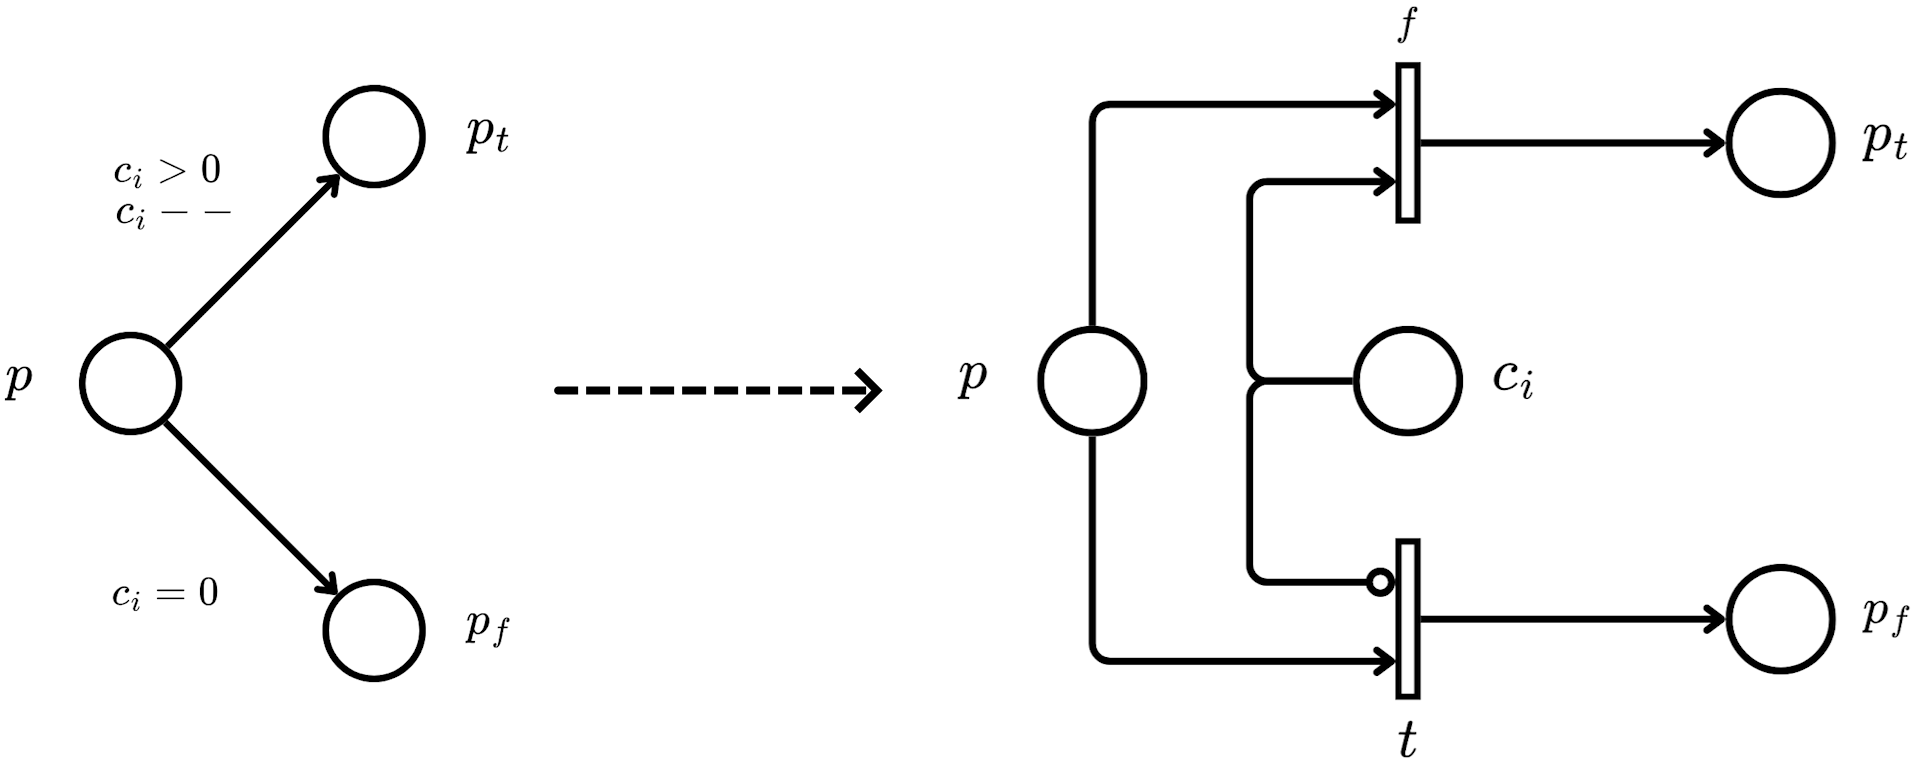
\includegraphics[width=0.85\linewidth]{img/minsky-machine-to-petri-net.png}
    \caption{Machine de Minsky implémentée en un réseau de Petri.}
    \label{fig:minsky-net}
\end{figure}

Pour simuler l'exécution d'une machine de Minsky $\mathcal{M} = (Q_{\mathcal{M}}, T_{\mathcal{M}}, c_1, c_2, \rho_0)$, on pose $P := Q_{\mathcal{M}} \cup \{c_1, c_2\}$ et $T := T_{\mathcal{M}}$. Ensuite, on définit $F$ de la manière suivante ; pour toute transition $t \in T_{\mathcal{M}}$ de $s$ à $s'$ : \begin{itemize}
    \item Si $t$ est un test à 0 sur $c_i$, alors $F(s, t) = F(t, s') = 1$ et $Inh(c_i, t) = 1$ d'où $F(c_i, t) = F(t, c_i) = 0$.
    \item Si $t$ décrémente $c_i$ après un test de positivité stricte, alors $F(s, t) = F(t, s') = F(c_i, t) = 1$.
    \item Si $t$ incrémente $c_i$, alors $F(s, t) = F(t, s') = F(t, c_i) = 1$.
\end{itemize}
On encode ensuite toute configuration $(q_k, i, j)$ de $\mathcal{M}$ dans un marquage $m \in \mathbb{Q}_+^{P}$ tel que : \begin{itemize}
    \item $m(q_k) = 1$ et $\forall l \neq k,\ m(q_l) = 0$.
    \item $m(c_i) = c_i$ (la valeur du compteur).
\end{itemize}

Cette construction pourrait fonctionner dans les réseaux discrets, comme on peut le voir dans la machine de Minsky implémentée dans un réseau de Petri (figure \ref{fig:minsky-net}). Or, notre réseau étant continu, nous devons l'améliorer afin d'assurer une exécution discrète.

Posons donc $\overline{\mathcal{N}} := (\overline{P}, \overline{T}, \overline{F}, \overline{m_0})$ le réseau de Petri continu qui simule des tirs discrets. L'idée est la suivante : on segmente chaque transition du réseau originel en un "sous-réseau" dans le réseau continu qui va forcer l'utilisation de tirs discrets. Basons-nous sur le réseau de la figure \ref{fig:petri-net}.

\begin{figure}[h]
    \centering
    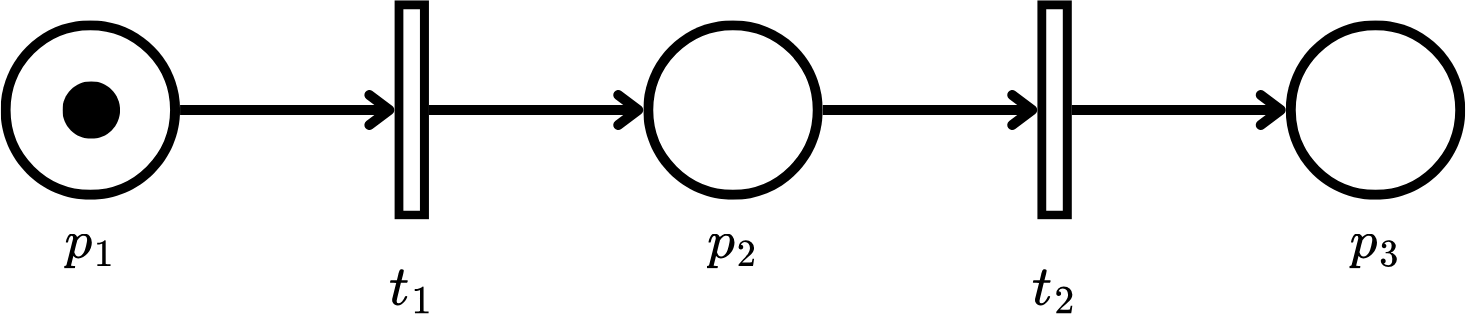
\includegraphics[width=0.45\linewidth]{img/petri-net.png}
    \caption{Réseau de Petri discret.}
    \label{fig:petri-net}
\end{figure}

Chaque sous-réseau de $\overline{\mathcal{N}}$ se base sur deux triplets $(q, ref(q), ref), (\overline{q}, \overline{ref(q)}, \overline{ref}) \in \overline{P} \times \overline{T} \times \overline{P}$ où $q, \overline{q}$ sont des places primordiales qui vont s'échanger un unique jeton à chaque tir d'une transition de $\overline{T}$ et ainsi garantir la discrétisation des marquages à l'aide de tests à 0.

Plus précisément, cet échange s'effectue en deux temps via $ref, \overline{ref}$ qui réceptionnent puis leur transfèrent leur contenu via les transitions $ref(q), \overline{ref(q)}$. Le choix de la place porteuse initiale du jeton entre $q$ et $\overline{q}$ est entièrement arbitraire. Supposons donc que $q$ a été choisie.

\begin{figure}[h]
    \centering
    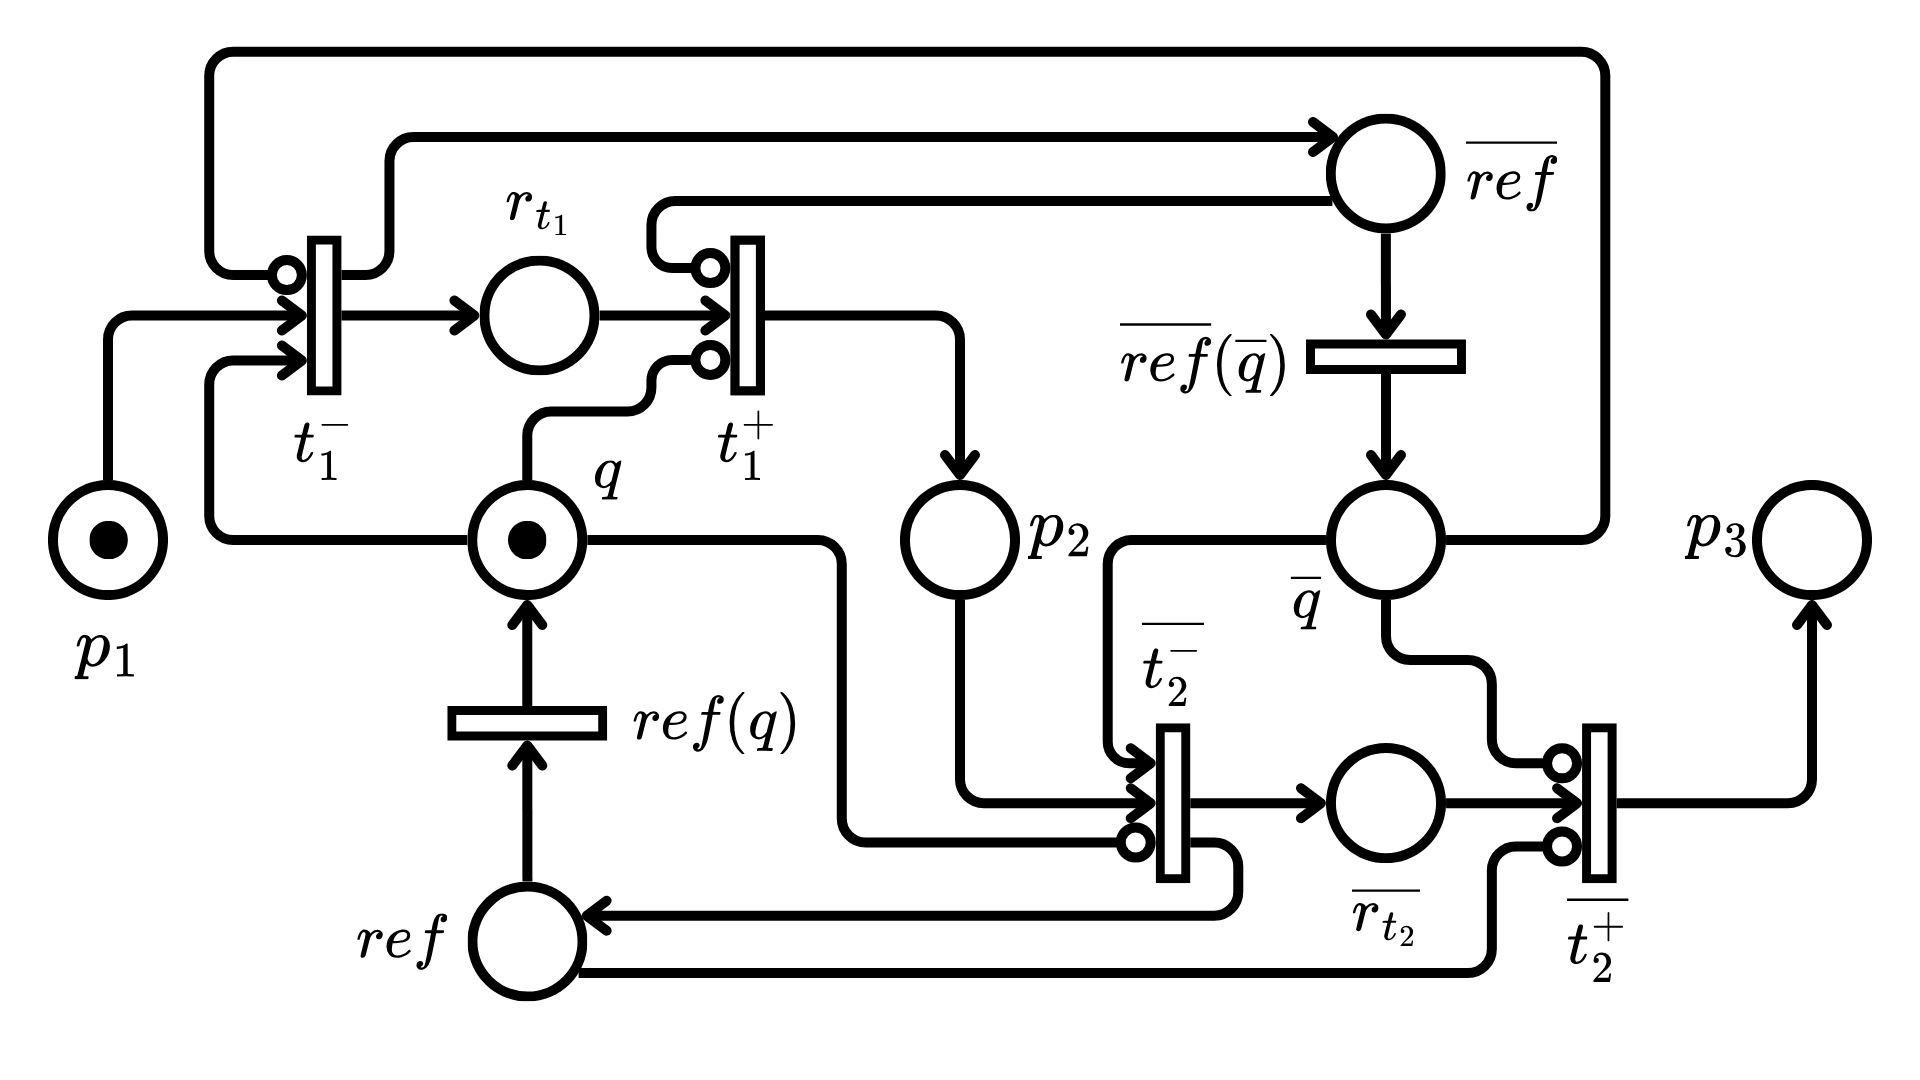
\includegraphics[width=0.75\linewidth]{img/continuous-petri-net.png}
    \caption{Réseau de Petri continu discrétisé de la figure \ref{fig:petri-net}.}
    \label{fig:continuous-petri-net}
\end{figure}

Pour chaque transition $t \in T$, on crée un triplet $(t^-, r_t, t^+) \in \overline{T} \times \overline{P} \times \overline{T}$ intermédiaire entre les places $\preb{t}$ et $\postb{t}$, et dont le fonctionnement repose sur l'utilisation du jeton dans $q$ et de son transfert progressif dans $\overline{q}$. En effet, un tir $\alpha \in \mathbb{Q} \setminus \mathbb{N}$ de $t^-$ agit sur l'ensemble des jetons dans les places de $\preb{t}$, mais aussi et surtout dans $q$ qui est contraint de transférer $\alpha$ jeton dans $\overline{q}$ via $t^-$ ; on en a tout autant dans $r_t$, la place intermédiaire entre $t^-$ et $t^+$. Ainsi, $t^+$ est bloquée par un arc inhibiteur $(q, t^+)$ qui empêche de poursuivre les tirs tant que $q$ n'est pas entièrement vidée : ceci laisse donc place à un marquage discret dans lequel on a un jeton dans $\overline{ref}$.

Désormais, $q$ est vide. Cependant, on veut d'abord remplir $\overline{q}$ avant de pouvoir tirer $t^+$ : c'est tout l'intérêt de l'arc inhibiteur $(\overline{ref}, t_1^+)$. On est donc contraints de transférer tous les jetons de $\overline{ref}$ à $\overline{q}$ en tirant $\overline{ref(q)}$, et l'on obtient à nouveau un marquage discret. On poursuit ainsi avec la partie suivante du réseau. La figure \ref{fig:continuous-petri-net} est un exemple d'une telle construction. Pour des raisons de visibilité, celle-ci a été simplifiée ; il faut garder à l'esprit que chaque triplet $(t^-, r_t, t^+)$ se basant sur $q$ a son équivalent symétrique $(\overline{t^-}, \overline{r_t}, \overline{t^+})$ se basant sur $\overline{q}$.

Posons alors $\overline{\mathcal{N}} := (\overline{P}, \overline{T}, \overline{F}, Inh, \overline{m_0})$, avec les composantes définies comme suit :
\begin{itemize}
    \item $\overline{P} := P \cup \{q, \overline{q}\} \cup \{ref, \overline{ref}\} \cup (\bigcup \limits_{t \in T} \{r_t, \overline{r_t}\})$
    \item $\overline{T} := \{ref(q), \overline{ref(q)}\} \cup (\bigcup \limits_{{t\in T}} \{t^-, t^+, \overline{t^-}, \overline{t^+}\})$
    \item $\overline{F}$ la relation de flots et $Inh$ la matrice indicatrice d'inhibition définies par, $\forall (p, t) \in P \times T$ : \begin{itemize}
        \item $\forall p' \in \preb{t},\ \overline{F}(p', t^-) = \overline{F}(p', \overline{t^-}) = F(p', t)$.
        \item $\forall p' \in \postb{t},\ \overline{F}(t^+, p') = \overline{F}(\overline{t^+}, p') = F(t, p')$.
        \item $\overline{F}(t^-, r_t) = \overline{F}(r_t, t^+) = \overline{F}(\overline{t^-}, \overline{r_t}) = \overline{F}(\overline{r_t}, \overline{t^+}) = 1$.
        \item $\overline{F}(q, t^-) = \overline{F}(\overline{q}, \overline{t^-}) = 1$.
        \item $\overline{F}(\overline{t^-}, ref) = \overline{F}(t^-, \overline{ref}) = 1$.
        \item $Inh(q, t^+) = Inh(\overline{ref}, t^+) = Inh(\overline{q}, \overline{t^+}) = Inh(ref, \overline{t^+}) = 1$.
    \end{itemize}
    \item $\begin{cases}
        \overline{m_0}(p) := m_0(p), \forall p \in P \\
        \overline{m_0}(r_t) = 0, \forall t \in T \\
        (\overline{m_0}(q), \overline{m_0}(\overline{q})) \in \{(1, 0), (0, 1)\}
    \end{cases}$
\end{itemize}

\begin{definition}
    Soit $t \in  T$ une transition. On dit que l'algorithme précédent discrétise $t$ dans $\overline{\mathcal{N}}$. De plus, si toute transition de $\mathcal{N}$ est discrétisée dans $\overline{\mathcal{N}}$, alors $\overline{\mathcal{N}}$ est la discrétisation de $\mathcal{N}$.
\end{definition}

\begin{definition}
    On définit l'ensemble $\runs[n]{\mathcal{M}}$ des exécutions de $\mathcal{M}$ de longueur $n \in \mathbb{N}$ par l'expression
    \[\runs[n]{\mathcal{M}} := \{\delta \in T_{\mathcal{M}}^n \mid \exists \rho \in C_{\mathcal{M}},\ \rho_0 \reaches[\delta] \rho\}.\]
\end{definition}

Notre objectif est désormais de prouver l'équivalence entre notre construction et les machines de Minsky. Pour ce faire, nous construisons deux applications : la première, $\Phi$, envoie toute configuration d'une machine de Minsky $\mathcal{M}$ en un marquage équivalent du réseau de Petri continu associé $\overline{\mathcal{N}}$ ; la deuxième, $\Psi$, envoie toute exécution $\delta \in \runs{M}$ dans une séquence de tirs $\sigma \in T^*$ de $\overline{\mathcal{N}}$.

\begin{definition}
    On définit l'application \[
        \function{\Phi}{C_{\mathcal{M}}}{\mathbb{N}^P}{(q_k, c_1, c_2)}{(0, \cdots, 0, \underbrace{1}_{q_k}, 0, \cdots, 0, \underbrace{n_1}_{c_1}, \underbrace{n_2}_{c_2}, \underbrace{n_q}_q, \underbrace{n_{\overline{q}}}_{\overline{q}})}
    \]
    qui envoie toute configuration $(q_k, c_1, c_2)$ d'une machine de Minsky $\mathcal{M}$ vers un marquage équivalent $m$ du réseau de Petri continu associé $\overline{\mathcal{N}}$.
\end{definition}

\begin{remark}
    $\Phi$ est injective. En effet, soient $\rho := (q_i, c_1, c_2),\ \rho' := (q_j, c_1', c_2') \in C_{\mathcal{M}}$ des configurations telles que $\Phi(\rho) = \Phi(\rho')$. En particulier : \begin{itemize}
        \item $\Phi(\rho)(q_i) = \Phi(\rho')(q_j)$, donc $q_i = q_j$.
        \item $\Phi(\rho)(c_1) = \Phi(\rho')(c_1')$, donc $c_1 = c_1'$.
        \item $\Phi(\rho)(c_2) = \Phi(\rho')(c_2')$, donc $c_2 = c_2'$.
    \end{itemize}
    En conclusion, $\rho = \rho'$.
\end{remark}

\begin{definition}
    On définit l'application \[
        \function{\Psi}{T_{\mathcal{M}}^*}{T^*}{(t_{\omega_1},\cdots,t_{\omega_n})}{(s_{\omega_1},\cdots,s_{\omega_n})}
    \]
    qui envoie toute exécution $(t_{\omega_1}, \cdots, t_{\omega_n})$ d'une machine de Minsky $\mathcal{M}$ vers une séquence de tirs du réseau de Petri continu associé $\overline{\mathcal{N}}$ où, pour tous $1 \leq i \leq n$, on a $s_{\omega_i} \in \{(t_{\omega_i}^-, ref(q), t_{\omega_i}^+), (\overline{t_{\omega_i}^-}, \overline{ref(q)}, \overline{t_{\omega_i}^+})\}$ avec $1 \leq \omega_i \leq n$, ce qui dépend du choix du porteur de jeton initial $q$ ou $\overline{q}$.
\end{definition}

\begin{remark}
    $\Psi$ n'admet bel et bien qu'une seule image pour toute exécution de $\mathcal{M}$ ; en effet, le choix du porteur de jeton initial $q$ ou $\overline{q}$ est fait par avance et devient donc fixe lors des tirs dans le réseau de Petri.
\end{remark}

\begin{lemma}
    \label{lemma:rational-lock}
    S'il existe un marquage accessible $m \in \creach{\overline{N}}{m_0}$ tel que $m(q) > 0$ et $m(\overline{q}) > 0$, alors pour tout marquage $m'$ tel que $m \creachess m'$, on a $m'(q) > 0$ et $m'(\overline{q}) > 0$.
\end{lemma}

\begin{proof}
    Posons $T_{\mathcal{N}} := \overline{T} \setminus \{ref(q), \overline{ref(q)}\}$. Par construction de $\overline{\mathcal{N}}$, pour toute transition $t \in T_{\mathcal{N}}$, on a soit $Inh(q, t) = 1$, soit $Inh(\overline{q}, t) = 1$. Or, comme $m(q), m(\overline{q}) > 0$, alors aucune transition de $T_{\mathcal{N}}$ ne peut être tirée. Sinon, si $m(ref) > 0$, alors on peut tirer $ref(q)$ et ainsi avoir un marquage $m' \geq m$ pour lequel on a donc $m'(q) > 0$. Le même raisonnement s'applique pour $\overline{ref}$ en tirant $\overline{ref(q)}$.
\end{proof}

\begin{lemma}
    \label{lemma:continuous-to-discrete-sequence}
    Pour tous marquages $m, m' \in \Phi(\reach{M}{\rho_0})$, s'il existe une séquence de tirs $\sigma \in (\mathbb{Q} \times T)^*$ telle que $m \creaches[\sigma] m'$, alors il existe une séquence de tirs discrets $\sigma' \in \Psi(\runs{\mathcal{M}})$ telle que $m \reaches[\sigma'] m'$.
\end{lemma}

\begin{proof}
    Soient $m, m' \in \Phi(\reach{M}{\rho_0})$. Supposons qu'il existe une séquence de tirs $\sigma \in (\mathbb{Q} \times T)^*$ telle que $m \creaches[\sigma] m'$. Sans perte de généralité, supposons également que $m(q) = 1$, d'où $m(\overline{q}) = 0$. Dans la disjonction de cas suivante, les séquences de tirs valides qui permettent donc de conclure sur l'accessibilité de $m'$ sont marqués par des crochets doubles $[\![\cdot]\!]$. Cela nous permettra de conclure plus aisément sur leur appartenance à $\Psi(\runs{\mathcal{M}})$.
    \begin{itemize}
        \item $\mathbf{(m \reaches[t_k^-] m_k^-)}$ : Par construction de $\Psi$, on a donc $p_k \in \overline{P}$ telle que $m(p_k) = 1$. Ainsi, par construction de $\overline{\mathcal{N}}$ également, on a $t_k^-$ sensibilisée. En tirant celle-ci avec $m \creaches[\alpha_k^- t_k^-] m_k^-$ où $0 < \alpha_k^- < 1$, on sait que $t_k^+$ ne peut être tirée à cause du test à 0 de l'arc inhibiteur $(q, t_k^+)$ ; or, $m_k^-(\overline{ref}) = \alpha_k^-$ et donc $\overline{ref(q)}$ est la seule transition nouvellement sensibilisée.
        En la tirant avec $m_k^- \creaches[\overline{\alpha_k^-}] \overline{m_k^-}$ où $0 < \overline{\alpha_k^-} \leq \alpha_k^-$, on aurait donc $\overline{m_k^-}(\overline{q}) = \overline{\alpha_k^-}$. Par le lemme \ref{lemma:rational-lock}, on débouche dans tous les cas suivants sur un marquage purement rationnel et donc $m'$ ne sera pas atteint. Supposons donc que $\alpha_k^- = 1$.
        \item $\mathbf{(m_k^- \reaches[\overline{ref(q)}] m_k^+)}$ : La seule transition nouvellement sensibilisée est ainsi $\overline{ref(q)}$ car $m_k^-(\overline{ref}) = 1$, ce qui empêche toujours $t_k^+$ d'être sensibilisée. En la tirant de sorte que $m_k^- \creaches[\overline{\alpha_k} \overline{ref(q)}] m_k^+$ où $0 < \overline{\alpha_k} < 1$, aucune transition n'est nouvellement sensibilisée. Supposons donc que $\overline{\alpha_k} = 1$.
        \item $\mathbf{[\![m_k^+ \creaches[\boldsymbol{\alpha}_k^+t_k^+] m_{k+1}]\!]}$ : On a donc $t_k^+$ nouvellement sensibilisée. En la tirant telle que $m_k^+ \creaches[\alpha_k^+ t_k^+] m_{k+1}$ où $0 < \alpha_k \leq 1$, il vient que $m_{k+1}(p_{k+1}) = \alpha_k^+$. Par conséquent, $\overline{t_{k+1}^-}$ est nouvellement sensibilisée. Si $\alpha_k^+ = 1$, alors $m_{k+1}$ est un marquage discret et l'on peut continuer ainsi par induction, d'où l'on atteindra finalement $m'$. Sinon, $0 < \alpha_{k}^+ < 1$ et il vient le sous-cas suivant.
        \item $\mathbf{(m_{k+1} \creaches[\boldsymbol{\alpha}_{k+1}^- \overline{t_{k+1}^-}] m_{k+1}^-)}$ : Comme $m_{k+1}(p_{k+1}) = \alpha_k^+$ et $m_{k+1}(\overline{q}) = 1$, alors $\overline{t_{k+1}^-}$ est sensibilisée. En tirant celle-ci telle que $m_{k+1} \creaches[\alpha_{k+1}^- \overline{t_{k+1}^-}] m_{k+1}^-$ où nécessairement $0 < \alpha_{k+1}^- \leq \alpha_k^+$, alors $m_{k+1}^-(\overline{r_{t_{k+1}^-}}) = m_{k+1}^-(ref) = \alpha_{k+1}^-$ et par conséquent, $ref(q)$ est nouvellement sensibilisée. Observons que si l'on tire cette dernière telle que $m_{k+1}^- \creaches[\overline{\alpha_{k+1}} ref(q)] \overline{m_{k+1}}$ où $0 < \overline{\alpha_{k+1}} \leq \alpha_{k+1}^-$ nécessairement, alors $\overline{m_{k+1}}(q), \overline{m_{k+1}}(\overline{q}) > 0$ et on obtiendra a fortiori une situation bloquante par le lemme \ref{lemma:rational-lock}. Supposons donc que l'on ne tire pas cette transition.
        \item $\mathbf{[\![m_{k+1} \reaches[\overline{t_{k+1}^-}] m_{k+1}^-]\!]}$ Ainsi, les seules transitions sensibilisées restantes sont $t_k^+, \overline{t_{k+1}^-}$ qui peuvent être tirées de façon alternée tant qu'a minima $t_k^+$ reste sensibilisée. L'ordre de ces tirs ne compte pas et peut ainsi être réorganisé de façon à ce que tous les tirs de $t_k^+$ soient effectués avant $\overline{t_{k+1}^-}$ ; il suffira de compresser chaque facteur en une somme inévitablement égale à 1. On obtient donc un marquage discret $m_{k+1}^+$ tel que $m_{k+1}^+(\overline{r_{t_{k+1}}}) = m_{k+1}^+(ref) = 1$ et le reste des places nul. On peut ainsi poursuivre par induction et finalement atteindre $m'$.
    \end{itemize}
    A fortiori, toutes les séquences de tirs sont de la forme \[\sigma = (t_1^-, ref(q), t_1^+, \cdots, s_l^-, ref_{s_l}(q_{s_l}), s_l^+) \in T^{3l},\ l \in \mathbb{N}\] où $(s_l^-, ref(q)_l, s_l^+) \in \{(t_l^-, ref(q), t_l^+), (\overline{t_l^-}, \overline{ref(q)}, \overline{t_l^+})\}$ suivant la parité de $l$. On en déduit que $\sigma \in \Psi(\runs{M})$ par construction. Un raisonnement analogue s'applique si le choix du porteur de jeton initial est $\overline{q}$. 
\end{proof}

Ainsi, nous tendons à prouver que les machines de Minsky sont équivalentes aux réseaux de Petri continus ainsi construits. Or, en réalité, il est encore impossible de le démontrer : notre réseau transforme les compteurs de la machine de Minsky en places, mais il est possible d'avoir une séquence alternée de tirs continus. On pourrait donc avoir un nombre purement rationnel de jetons dans ces places, ce qui pourrait fausser le comportement de l'implémentation de notre machine de Minsky. Nous allons donc construire une machine de Minsky $\overline{\mathcal{M}}$ trivialement équivalente à $\mathcal{M}$.

Tout d'abord, soit $q \in Q_{\mathcal{M}}$ un état. S'il existe une transition labellisée $t \in T_{\mathcal{M}}$ telle que $q \in \postb{t}$ et $t$ change la valeur d'un compteur de $\mathcal{M}$, alors on dit que $q$ est \textit{variante}. Ainsi, pour toute place variante $q$ de $\mathcal{M}$, on construit dans $\overline{\mathcal{M}}$ une place $q'$ dite de \textit{stabilisation}. Ainsi, dans $\overline{\mathcal{M}}$, $q'$ "absorbe" les transitions entrantes de $q$ dans $\mathcal{M}$, c'est-à-dire $\preb{q'} := \preb{q}$, et la seule transition sortante de $q'$ et entrante dans $q$ devient $t_q$, permettant de passer de $q'$ à $q$ sans modification du compteur : on définit donc $\postb{q'}, \preb{q} := \{t_q\}$. Le reste des transitions et des places reste parfaitement intact. Ce nouvel état permet donc de stabiliser les compteurs dans $\overline{\mathcal{N}}$. Ainsi, comme les nouvelles transitions n'affectent pas le comportement de l'ancienne machine sur les compteurs ni ne modifient autrement que par la longueur les exécutions de $\mathcal{M}$, nous affirmons que $\overline{\mathcal{M}}$ est équivalente à $\mathcal{M}$. Dans les paragraphes suivants, nous admettons que les machines de Minsky ont la forme de $\overline{\mathcal{M}}$ et on suppose que l'on a donc : \begin{itemize}
    \item Une machine de Minsky $\mathcal{M} := (Q_{\mathcal{M}}, T_{\mathcal{M}}, c_1, c_2, \rho_0)$ où $Q_{\mathcal{M}} := \{q_0, \cdots, q_m\},\ m \in \mathbb{N}$ et $\rho_0 = (q_0, 0, 0)$.
    \item Un réseau de Petri continu à arcs inhibiteurs $\mathcal{N} := (P, T, F, Inh, m_0)$ simulant $\mathcal{M}$ où donc $m_0 := \Phi(\rho_0)$.
\end{itemize}

% \begin{property}
%     Soient $(m_1, \sigma, m_2) \in \mathbb{N}^{\overline{P}} \times T \times \mathbb{N}^{\overline{P}}$ tels que $m_1 \reaches[\sigma] m_2$. S'il existe $\rho_1 \in C_{\mathcal{M}},\ t \in T_{\mathcal{M}}$ tels que $m_1 = \Phi(\rho_1)$ et $\sigma = \Psi(t)$, alors il existe $\rho_2 \in C_{\mathcal{M}}$ tel que $m_2 = \Phi(\rho_2)$.
% \end{property}

La propriété suivante est fondamentale. En effet, elle garantit que toute configuration de $\mathcal{M}$ adaptée en marquage $m$ dans $\mathcal{N}$ débouchera sur un marquage $m'$ de la même forme, en prenant en compte que les transitions tirées pour passer de $m$ à $m'$ sont précisément des exécutions de $\mathcal{M}$.

\begin{property}
    \label{property:minsky-preservation}
    Soient : \begin{itemize}
        \item $(\rho_1, t, \rho_2) \in C_{\mathcal{M}} \times T_{\mathcal{M}} \times C_{\mathcal{M}}$ tels que $\rho_1 \reaches[t] \rho_2$.
        \item $(m_1, \Psi(t), m_2) \in \mathbb{N}^P \times T \times \mathbb{N}^P$ tels que $m_1 \reaches[\Psi(t)] m_2$.
    \end{itemize}
    Si $m_1 = \Phi(\rho_1)$, alors $m_2 = \Phi(\rho_2)$.
\end{property}

\begin{proof}
    Supposons que $m_1 = \Phi(\rho_1)$. Par hypothèse, on sait que : \begin{itemize}
        \item $m_1$ est de la forme $(0, \cdots, 0, q_k, 0, \cdots, 0, c_1, c_2, q, \overline{q})$ avec $(m_1(q), m_1(\overline{q})) \in \{(0, 1), (1, 0)\}$.
        \item $\Psi(t)$ est de la forme $(t^-, ref_t(q_t), t^+) \in T^3$ où $ref_t(q_t) \in \{ref(q), \overline{ref(q)}\}$.
    \end{itemize}
    Supposons sans perte de généralité que $m_1(q) = 1$. Ainsi, la seule transition sensibilisée est $t_k^-$ où nécessairement $q_k \in \preb{t_k^-}$. On en déduit que $t^- = t_k^-$. On aboutit à un marquage $m_1^-$ tel que $m_1^-(\overline{ref(q)}) = m_1^-(r_{t_k}) = 1$ et donc $m_1^-(q_k) = 0$. La seule transition sensibilisée est désormais $\overline{ref(q)}$, par conséquent $ref_t(q_t) = \overline{ref(q)}$. On aboutit à un marquage $m_1^+$ tel que $m_1^+(\overline{q}) = 1$ et $m_1^+(\overline{ref(q)}) = 0$. Ainsi, $t_k^+$ est la seule transition sensibilisée, donc $t^+ = t_k^+$. Il s'en suit donc que $\Psi(t) = (t_k^-, \overline{ref(q)}, t_k^+)$ qui débouche sur un marquage $m_2$ tel que $m_2(q_{k+1}) = m_2(\overline{q}) = 1$ et $m_2(r_{t_k}) = 0$ : cela revient précisément à dire que $m_2 = \Phi(r_{t_k})$.
\end{proof}

\begin{remark}
    Cette propriété s'applique également sur des exécutions d'une longueur supérieure à 1.
\end{remark}

Maintenant, on peut démontrer le lemme qui suit à l'aide de la propriété précédente. Celui-ci garantit que toute exécution qui tire les transitions de $\mathcal{N}$ par paquets de 3 représente alors une exécution de notre machine de Minsky.

\begin{lemma}
    \label{lemma:seq-to-run}
    Soit $n \in \mathbb{N},\ \sigma \in T^{3n}$ une séquence de tirs discrets. Si $m_0 \reaches[\sigma] m$, alors il existe une unique exécution $\delta \in \runs[n]{M}$ telle que $\sigma = \Psi(\delta)$.
\end{lemma}

\begin{proof}
    \natinduction{P}{\mathbb{N}}{\forall \sigma \in T^{3n},\ m_0 \reaches[\sigma] m \Longrightarrow \exists ! \delta \in \runs[n]{M},\ \sigma = \Psi(\delta)}{
        Soit $\sigma_0$ la séquence vide. Posons l'unique exécution vide $\delta_0$. Alors trivialement, $\sigma_0 = \Psi(\delta_0)$.
    }{
        Soit $\sigma_{n+1} \in T^{3(n+1)}$ tel que $m_0 \reaches[\sigma_{n+1}] m_{n+1}$.
        Alors on a $\sigma_n \in T^{3n},\ (s_1, s_2, s_3) \in T^3,\ m_n \in \mathbb{N}^P$ tels que $m_0 \reaches[\sigma_n] m_n \reaches[s_1s_2s_3] m_{n+1}$. Par hypothèse de récurrence, on a un unique $\delta_n \in \runs[n]{M}$ tel que $\sigma_n = \Psi(\delta_n)$. Par définition de $\delta_n$, on a donc une configuration $\rho_n \in C_{\mathcal{M}}$ telle que $\rho_0 \reaches[\delta_n] \rho_n$. De plus, par la propriété \ref{property:minsky-preservation}, comme $m_0 = \Phi(\rho_0)$ et $m_0 \reaches[\sigma_n] m_n$, il vient que $m_n = \Phi(\rho_n)$. Par construction de $\Phi$, on a donc une unique place $q_{\omega_n} \in \{q_i : i \in [\![0, m]\!]\}$ telle que $m_n(q_{\omega_n}) = 1$. Supposons sans perte de généralité que $m_n(q) = 1$.
        \begin{enumerate}
            \item $(m_n \reaches[s_1 = t_{\omega_n}^-] m_n^-)$. L'unique transition sensibilisée en ce cas est $t_{\omega_n}^-$, d'où nécessairement $s_1 = t_{\omega_n}^-$. On obtient un marquage $m_n^-$ tel que $m_n^-(r_{s_1}) = m_n^-(\overline{ref(q)}) = 1$.
            \item $(m_n^- \reaches[s_2 = ref(q)] m_n^+)$. À nouveau, l'unique transition sensibilisée est $\overline{ref(q)}$, d'où $s_2 = \overline{ref(q)}$. En la tirant, on obtient un marquage $m_n^+$ tel que $m_n^+(\overline{q}) = 1$.
            \item $(m_n^+ \reaches[s_3 = t_{\omega_n}^+] m_{n+1})$. Enfin, l'unique transition sensibilisée est donc $t_{\omega_n}^+$. On en déduit que $s_3 = t_{\omega_n}^+$, d'où l'on obtient le marquage $m_{n+1}$.
        \end{enumerate}
        On remarque que $\sigma_{end} = (s_1, s_2, s_3) \in \Psi(T_{\mathcal{M}}^*)$, donc on a un unique $\delta_{end} \in T_{\mathcal{M}}^3$ tel que $\Psi(\delta_{end}) = \sigma_{end}$. En posant $\delta_{n+1} := \delta_n \delta_{end} \in \runs[n+1]{M}$, alors $\delta_{n+1}$ est unique et en particulier, comme $\Psi(\delta_n) = \sigma_n$ et $\Psi(\delta_{end}) = \sigma_{end}$, alors $\Psi(\delta_{n+1}) = \sigma_{n+1}$.
    }
\end{proof}

Notre objectif est désormais de démontrer le lemme \ref{lemma:sequence-unwrap-to-execution} qui permet de passer d'un marquage représentant une configuration de $\mathcal{M}$ à la configuration elle-même. Pour ce faire, nous avons besoin de prouver dans un premier temps que la simulation du tir d'une transition labellisée de $\mathcal{M}$ dans notre réseau $\mathcal{N}$ est correcte : c'est le dessein de la propriété \ref{property:exec-to-run}. Puis, nous montrons via la proposition \ref{proposition:triplet-sequence} que n'importe quelle séquence de tirs débouchant sur un marquage ayant la forme d'une configuration de $\mathcal{M}$ est nécessairement effectuée par paquets de 3. De cette façon, nous nous appuyons sur le lemme précédent qui nous permet de conclure sur l'existence d'une exécution correcte de notre machine $\mathcal{M}$.

\begin{property}
    \label{property:exec-to-run}
    Soient $(\rho_1, t, \rho_2) \in C_{\mathcal{M}} \times T_{\mathcal{M}} \times C_{\mathcal{M}}$. Si $\Phi(\rho_1) \reaches[\Psi(t)] \Phi(\rho_2)$, alors $\rho_1 \reaches[t] \rho_2$.
\end{property}

\begin{proof}
    Supposons par l'absurde que $\Phi(\rho_1) \reaches[\Psi(t)] \Phi(\rho_2)$ et $\rho_1 \reaches[t] \rho_2'$ où $\rho_2 \neq \rho_2'$. Par la propriété $\ref{property:minsky-preservation}$, on obtient que $\Phi(\rho_2) = \Phi(\rho_2')$. Par injectivité de $\Phi$, on en déduit que $\rho_2 = \rho_2'$, contradiction.
\end{proof}

\begin{proposition}
    \label{proposition:triplet-sequence}
    Soit $m \in \mathbb{N}^P$ un marquage tel que $m_0 \reaches[\sigma] m$ avec $\sigma \in T^*$. S'il existe une configuration $\rho \in C_{\mathcal{M}}$ telle que $m = \Phi(\rho)$, alors $|\sigma| \equiv 0\ [3]$.
\end{proposition}

\begin{proof}
    Supposons qu'il existe $\rho \in C_{\mathcal{M}}$ telle que $m = \Phi(\rho)$ et $|\sigma| \not\equiv 0\ [3]$. Supposons également sans perte de généralité que $\sigma = (t_{\omega_1}, \cdots, t_{\omega_n}),\ n \in \mathbb{N}$ et que $q$ est le porteur de jeton initial. De toute évidence, comme $m_0 = \Phi(\rho_0)$, alors $n \geq 1$.
    En commençant donc à $m_0 = (1, 0, \cdots, 0, c_1, c_2, 1, 0)$, on sait que la seule transition sensibilisée est $t_0^-$. Ainsi, $t_{\omega_1} = t_0$. Le marquage $m^-$ ainsi obtenu n'est pas dans l'image de $\Phi$ car $m^-(\overline{ref(q)}) = 1$. Ainsi, $m^- \neq m$ et $n \geq 2$.
    La seule transition sensibilisée suivante est donc $\overline{ref(q)}$. Ainsi, $t_{\omega_2} = \overline{ref(q)}$. Le marquage $m^+$ ainsi obtenu n'est toujours pas dans l'image de $\Phi$ car $m^+(r_t) = 1$. Ainsi, $m^+ \neq m$ et $n \geq 3$.
    Enfin, la seule transition sensibilisée à cet instant est $t_0^+$. Ainsi, $t_{\omega_3} = t_0^+$. Le marquage $m_1 = (0, 1, 0, \cdots, 0, c_1, c_2, 0, 1)$ ainsi obtenu est donc dans l'image de $\Phi$, or $n = 3 \equiv 0\ [3]$ en ce cas. Par récurrence immédiate, on a une contradiction dans tous les cas.
\end{proof}

\begin{lemma}
    \label{lemma:sequence-unwrap-to-execution}
    Soit $\rho \in C_{\mathcal{M}}$ une configuration. Si $\Phi(\rho) \in \reach{N}{m_0}$, alors $\rho \in \reach{M}{\rho_0}$.
\end{lemma}

\begin{proof}
    Supposons que $\Phi(\rho) \in \reach{N}{m_0}$. Alors il existe une séquence de tirs $\sigma \in T^*$ telle que $m_0 \reaches[\sigma] \Phi(\rho)$. Comme $m_0 \reaches[\sigma] \Phi(\rho)$, alors $|\sigma| \equiv 0\ [3]$ par la proposition \ref{proposition:triplet-sequence}. Ainsi, il existe une unique exécution $\delta$ telle que $\Psi(\delta) = \sigma$ par le lemme \ref{lemma:seq-to-run}. On a donc que $m_0 = \Phi(\rho_0) \reaches[\sigma = \Psi(\delta)] \Phi(\rho)$. On en conclut que $\rho_0 \reaches[\delta] \rho$ par la propriété \ref{property:exec-to-run}, d'où $\rho \in \reach{M}{\rho_0}$.
\end{proof}

Enfin, le théorème suivant appuie l'équivalence entre notre réseau et notre machine de Minsky. La condition suffisante est prouvée par récurrence en la longueur des exécutions de $\mathcal{M}$. En revanche, la condition nécessaire est prouvée directement en nous appuyant sur les lemmes \ref{lemma:continuous-to-discrete-sequence} et \ref{lemma:sequence-unwrap-to-execution}, qui permettent d'aboutir élégamment au résultat tant recherché.

\begin{theorem}
    Soit $\rho_{\omega_n} = (q_n, i_{\omega_n}, j_{\omega_n}) \in C_{\mathcal{M}}$ une configuration avec $n \leq m$ et $i_{\omega_n}, j_{\omega_n} \in \mathbb{N}$. Alors
    \[\rho_{\omega_n} \in \reach{M}{\rho_0} \Longleftrightarrow \Phi(\rho_{\omega_n}) \in \creach{N}{\Phi(\rho_0)}.\]
\end{theorem}

\begin{proof}
    \textbf{Condition suffisante.} \natinduction{P}{\mathbb{N}}{\rho_{\omega_n} \in \reach[n]{M}{\rho_0} \Longrightarrow \Phi(\rho_{\omega_n}) \in \creach[3n]{N}{\Phi(\rho_0)}}{
        Trivialement, si $\rho_0 \in \reach[0]{M}{\rho_0}$, alors $\Phi(\rho_0) \in \reach[0]{N}{\Phi(\rho_0)}$ car aucune transition n'est tirée.
    }{\\
        Soit $\rho_{n+1} \in \reach[n+1]{M}{\rho_0}$.
        \begin{itemize}
            \item \textbf{(Compteurs constants.)} Supposons donc dans un premier temps que le passage de $q_n$ à $q_{n+1}$ ne change pas la valeur des compteurs.
            Alors $\postb{t_n}$ ne contient aucune place variante.
            On a une séquence de transitions labellisées $(t_k)_{k \leq n}$ telles que $\rho_0 \reaches[t_0] \cdots \reaches[t_{n-1}] \rho_n \reaches[t_n] \rho_{n+1}$ avec $\rho_n := (q_n, i_n, j_n),\ \rho_{n+1} := (q_{n+1}, i_{n+1}, j_{n+1})$, d'où l'on a $\rho_n \in \reach[n]{M}{\rho_0}$ et par hypothèse de récurrence, $\Phi(\rho_n) \in \creach[3n]{N}{\Phi(\rho_0)}$.
            Supposons que $\Phi(\rho_n)(q) = 1$.
            Par construction de $\mathcal{N}$, $t_n$ est implémentée par un ensemble de transitions $\{t_n^-, t_n^+\}$.
            Alors on tire $\sigma = (t_n^-, \overline{ref(q)}, t_n^+) \in T^3$.
            On obtient ainsi un marquage $m_{n+1}$ tel que $m_{n+1}(q_n) = 0$ et $m_{n+1}(q_{n+1}) = 1$.
            Par hypothèse, les transitions $[\![\sigma]\!]$ n'ont pas d'effet sur les compteurs $(c_1, c_2)$, donc $m_{n+1}(c_1) = i_{n+1}$ et $m_{n+1}(c_2) = j_{n+1}$.
            De plus, $3n + 3 = 3(n+1)$ transitions ont été franchies au total.
            Ainsi, $m_{n+1} = \Phi(\rho_{n+1})$ et comme $\Phi(\rho_0) \reachess \Phi(\rho_n) \reaches[\sigma] \Phi(\rho_{n+1})$, alors $\Phi(\rho_{n+1}) \in \reach[3(n+1)]{N}{\Phi(\rho_0)}$.
            Un raisonnement analogue est applicable si $\Phi(\rho_n)(\overline{q}) = 1$.
            \item \textbf{(Compteurs modifiés.)} Supposons désormais que le passage de $q_n$ à $q_{n+1}$ change la valeur des compteurs.
            Alors $q_n$ est une place variante et une place de stabilisation $q_n'$ a été implémentée dans $\mathcal{M}$.
            Ainsi, pour passer de $q_n$ à $q_{n+1}$, deux transitions $t_n$ et $t_n'$ ont été tirées.
            On a donc une séquence de transitions labellisées $(t_k)_{k \leq n}$ telles que $\rho_0 \reaches[t_0] \cdots \reaches[t_{n-2}] \rho_n' \reaches[t_{n-1}] \rho_n \reaches[t_n] \rho_{n+1}$ avec $\rho_n' := (q_n', i_n, j_n),\ \rho_n := (q_n, i_n, j_n),\ \rho_{n+1} := (q_{n+1}, i_{n+1}, j_{n+1})$, d'où l'on a $\rho_n \in \reach[n]{M}{\rho_0}$ et par hypothèse de récurrence, $\Phi(\rho_n) \in \creach[3n]{N}{\Phi(\rho_0)}$.
            Par un raisonnement analogue au paragraphe précédent, on en conclut que $\Phi(\rho_{n+1}) \in \reach[3(n+1)]{N}{\Phi(\rho_0)}$.
            % Supposons que $\Phi(\rho_n)(q) = 1$.
            % Par construction de $\mathcal{N}$, $t_n$ est implémentée par un ensemble de transitions $\{t_n^-, t_n^+, \overline{t_n^-}', \overline{t_n^+}'\}$.
            % Alors on tire $\sigma = (t_n^-, \overline{ref(q)}, t_n^+, \overline{t_n^-}', ref(q), \overline{t_n^+}') \in T^6$.
            % On obtient ainsi un marquage $m_{n+1}$ tel que $m_{n+1}(q_n) = 0$ et $m_{n+1}(q_{n+1}) = 1$.
            % Les transitions $[\![\sigma]\!]$ conservent l'action de $t_n$ dans $\mathcal{M}$ sur les compteurs $(c_1, c_2)$, donc $m_{n+1}(c_1) = i_{n+1}$ et $m_{n+1}(c_2) = j_{n+1}$.
            % De plus, $k + 6$ transitions ont été franchies au total, d'où $3n + 6 \leq k + 6 \leq 6n + 6 \Longrightarrow 3(n+1) \leq k' \leq 6(n+1)$ avec $k' := k + 6$.
            % Ainsi, $m_{n+1} = \Phi(\rho_{n+1})$ et comme $\Phi(\rho_0) \reachess \Phi(\rho_n) \reaches[\sigma] \Phi(\rho_{n+1})$, alors $\Phi(\rho_{n+1}) \in \reach[k']{N}{\Phi(\rho_0)}$.
            % Un raisonnement analogue est applicable si $\Phi(\rho_n)(\overline{q}) = 1$.
        \end{itemize}
        \textbf{Condition nécessaire.} Supposons que $\Phi(\rho_{\omega_n}) \in \creach{N}{\Phi(\rho_0)}$.
        Alors il existe une séquence de tirs $\sigma \in (\mathbb{Q} \times T)^*$ telle que $\Phi(\rho_0) \creaches[\sigma] \Phi(\rho_{\omega_n})$.
        Par le lemme \ref{lemma:continuous-to-discrete-sequence}, il existe une séquence de tirs discrets $\sigma' \in \Psi(\runs{M})$ telle que $\Phi(\rho_0) \reaches[\sigma'] \Phi(\rho_{\omega_n})$, d'où $\Phi(\rho_{\omega_n}) \in \reach{N}{\Phi(\rho_0)}$.
        Or, par le lemme \ref{lemma:sequence-unwrap-to-execution}, on en déduit que $\rho_{\omega_n} \in \reach{M}{\rho_0}$.
    }
\end{proof}

Comme l'arrêt d'une machine de Minsky est indécidable, il est désormais clair que l'apparition des arcs inhibiteurs dans nos réseaux de Petri continus rend ce même caractère à la propriété d'accessibilité.

\subsection{Implémentation d'arcs de reset}

Dans cette section, nous nous intéressons à l'ajout d'arcs de reset à nos réseaux de Petri continus. On pose leur sémantique dans la définition suivante.

\begin{definition}
    Un réseau de Petri continu à arcs de reset est un quintuplet $\mathcal{N} := (P, T, F, Inh, m_0)$ où : \begin{itemize}
        \item $(P, T, F, m_0)$ est un réseau de Petri continu.
        \item $Inh$ est une matrice indexée par $P \times T$ à coefficients dans $\{0, 1\}$ telle que, pour tous $(p, t) \in  P \times T$ : \[\begin{cases}
            Inh(p, t) = 1 & \text{si } (p, t) \text{ est inhibiteur.} \\
            Inh(p, t) = 0 & \text{sinon.}
        \end{cases}\]
        Ainsi, si $Inh(p, t) = 1$, alors nécessairement $F(p, t) = F(t, p) = 0$.
    \end{itemize}
\end{definition}

Nous nous penchons alors sur le problème d'accessibilité en nous inspirant des travaux de \cite{dufourd} dans leurs réseaux de Petri classiques. Ces derniers reconstruisent le réseau en s'appuyant sur la création de places jumelles $p'$ pour toute place $p$ impliquée dans le test à 0 d'un arc inhibiteur : c'est une place inhibitrice. Soit donc $\mathcal{N} = (P, T, F, Inh, m_0)$ un réseau de Petri à arcs inhibiteurs. On pose
\begin{equation*}
    \function{\indicator_{Inh}}{P}{\{0, 1\}}{p}{\begin{cases}
        1 & \text{si } \exists t \in T,\ Inh(p, t) = 1. \\
        0 & \text{sinon.}
    \end{cases}}
\end{equation*}
la fonction indicatrice d'inhibition et $\mathbb{I}_{\mathcal{N}} := \indicator_{Inh}^{-1}(\{1\}) = \{p \in P \mid \indicator_{Inh}(p) = 1\}$ l'ensemble des places inhibitrices de $\mathcal{N}$. Ils définissent $\mathcal{N}^+ := (P^+, T, F^+, Res, m_0^+)$ le réseau de Petri jumeau à arcs de reset où : \begin{enumerate}
    \item $P^+ := P \cup P'$, où $P' := \{p' : p \in \mathbb{I}_{\mathcal{N}}\}$ (avec $P \cap P' = \emptyset$).
    \item La relation de flots $F^+$ est définie, $\forall (p, t) \in P \times T$, par : \[\begin{cases}
        F^+(p, t) = F^+(t, p') = 0 & \text{si } Inh(p, t) = 1.\\
        F^+(p, t) := F(p, t),\ F^+(t, p) := F(t, p) & \text{sinon.}
    \end{cases}\]
    \item On étend les marquages de $\mathcal{N}$ à $\mathcal{N^+}$ par l'application \begin{equation*}
        \function{\extend}{\mathbb{Q}^P}{\mathbb{Q}^{P^+}}{(p_1, \cdots, p_n)}{(p_1, \cdots, p_n, p'_{\omega_1}, \cdots, p'_{\omega_k})}
    \end{equation*}
    avec $1 \leq \omega_1 < \cdots < \omega_k \leq n,\ k \leq n$ où les places distinctes $p'_{\omega_i}$ sont les jumelles de places $p_{\omega_i}$.
    \item On pose $Res \in \mathcal{M}_{P^+ \times T}(\{0, 1\})$ la matrice de reset telle que, pour tous $(p, t) \in P \times T$, \begin{itemize}
        \item $Res(p, t) = 0$.
        \item $Res(p', t) = \begin{cases}
            p' & \text{si } Inh(p, t) = 1 \\
            0  & \text{sinon.}
        \end{cases}$
    \end{itemize}
    \item Pour tout tir $m \creaches[\alpha t] m'$, on redéfinit l'équation caractéristique de la manière suivante : \[m' = m + \alpha C(t) - Res(t)\]
\end{enumerate}

La figure \ref{fig:reset-arc-petri-net} nous montre un exemple concret d'une telle construction.
\begin{figure}[ht]
    \centering
    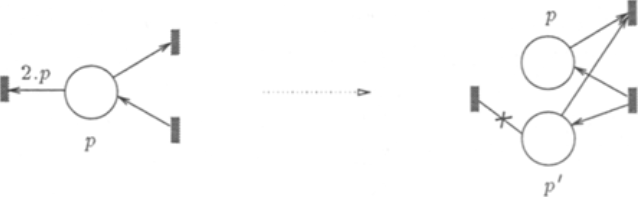
\includegraphics[width=0.5\linewidth]{img/reset-arc-petri-net.png}
    \caption{Transformation d'un réseau à arcs inhibiteurs en réseau à arcs de reset par \cite{dufourd}.}
    \label{fig:reset-arc-petri-net}
\end{figure}
La relation de flots avec tout arc de $p$ est donc reproduite à l'identique pour $p'$, à l'exception de l'arc inhibiteur dont la liaison avec $p$ est retirée pour la transformer en arc de reset sur $p'$.

Nous allons prouver que ces deux structures sont isomorphes en nous appuyant sur l'algèbre linéaire. Pour commencer, nous admettons la proposition suivante (qui peut être démontrée) :

\begin{proposition}
    $\mathbb{Q}^P$ est un $\mathbb{Q}$-espace vectoriel de dimension $|P|$.
\end{proposition}

Reprenons alors notre définition de $\extend$, et montrons les propriétés suivantes.

\begin{property}
    L'application $\extend$ est linéaire sur $\mathbb{Q}^P$.
\end{property}

\begin{proof}
    Soient $x = (x_1, \cdots, x_n),\ y = (y_1, \cdots, y_n) \in \mathbb{Q}^P,\ \alpha \in \mathbb{Q}$.
    Alors \begin{align*}
        \extend[\alpha x + y] & = \extend[(\alpha x_1 + y_1, \cdots, \alpha x_n + y_n)] \\
                              & = (\alpha x_1 + y_1, \cdots, \alpha x_n + y_n, (\alpha x_{\omega_1} + y_{\omega_1})', \cdots, (\alpha x_{\omega_k} + y_{\omega_k})') \\
                              & = (\alpha x_1 + y_1, \cdots, \alpha x_n + y_n, \alpha x'_{\omega_1} + y'_{\omega_1}, \cdots, \alpha x'_{\omega_k} + y'_{\omega_k}) \\
                              & = \alpha(x_1, \cdots, x_n, x'_{\omega_1}, \cdots, x'_{\omega_k}) + (y_1, \cdots, y_n, y'_{\omega_1}, \cdots, y'_{\omega_k}) \\
                              & = \alpha \extend[x] + \extend[y].
    \end{align*}
\end{proof}

\begin{property}
    L'application $\extend[\cdot]$ est injective.
\end{property}

\begin{proof}
    Soient $m_1, m_2 \in \mathbb{Q}^P$ tels que $\extend[m_1] = \extend[m_2]$.
    Trivialement, $\forall p \in P$, \[m_1(p) = \extend[m_1](p) = \extend[m_2](p) = m_2(p),\] d'où $m_1 = m_2$.
\end{proof}

Remarquons que tout marquage $m^+$ dans $\mathcal{N}^+$ est défini via un marquage $m$ de $\mathcal{N}$. Cela signifie qu'un tir de reset d'une place non vide $p^+ \in P^+$ dans $\mathcal{N^+}$ est irrécupérable dans $\mathcal{N}$, et donc le marquage obtenu n'a aucun équivalent dans ce dernier. On s'intéresse donc seulement à l'ensemble $\extend[\mathbb{Q}^P] \subseteq \mathbb{Q}^{P^+}$, c'est-à-dire les extensions des marquages de $\mathcal{N}$. Posons maintenant $\prototype{\coextend}{\mathbb{Q}^P}{\extend[\mathbb{Q}^P]}$ la corestriction de $\extend$ à $\mathbb{Q}^P$. Il vient la propriété suivante.

\begin{proposition}
    L'application $\coextend$ est un isomorphisme entre $\mathbb{Q}^P$ et $\extend[\mathbb{Q}^P]$.
\end{proposition}

\begin{proof}
    Restreindre l'ensemble d'arrivée de $\extend$ ne change en rien son caractère linéaire et injectif. De plus, la corestriction $\restrict{f}{f(E)}$ de toute application $\prototype{f}{E}{F}$ est surjective par définition. Ainsi, $\coextend$ est injective et surjective, donc bijective. Comme elle est également linéaire, alors on en déduit qu'il s'agit d'un isomorphisme.
\end{proof}

\begin{remark}
    Pour tout marquage $m^+ \in \extend[\mathbb{Q}^P]$, il existe donc un unique marquage $m \in \mathbb{Q}^P$ tel que $\coextend[m] = m^+$. En ce cas, on note également $\rcoextend[m^+] = m$.
\end{remark}

Nous avons donc un isomorphisme $\coextend$ entre les marquages de $\mathbb{Q}^P$ et de $\extend[\mathbb{Q}^P]$. Or, nous nous intéressons aux marquages \textit{accessibles} dans $\mathcal{N}$ et $\mathcal{N}^+$ respectivement depuis $m_0$ et $m_0^+$, ce qui correspond respectivement aux ensembles $\creach{N}{m_0}$ et $\creach{N^+}{m_0^+} = \extend[\creach{N}{m_0}]$. Nous voulons donc prouver que ces deux réseaux ont exactement les mêmes comportements. Nous nous appuierons sur les équations caractéristiques de chaque réseau, qui reposent sur leurs matrices d'incidence $C$ et $C^+$, c'est pourquoi nous commençons par prouver le lemme suivant qui nous permettra de reconstruire les chemins dans chaque réseau et d'établir une équivalence entre les deux.

\begin{lemma}
    \label{lemma:net-balance-preservation}
    Soient : \begin{itemize}
        \item $(m_1, m_1^+) \in \creach{N}{m_0} \times \extend[\creach{N}{m_0}]$ des marquages accessibles.
        \item $(m_2, m_2^+) \in \mathbb{Q}_+^P \times \extend[\mathbb{Q}_+^P]$ des marquages tels que $\coextend[m_2] = m_2^+$.
        \item $(\alpha, t) \in \mathbb{Q}_+ \times T$ un tir tel que $m_1 \creaches[\alpha t] m_2$ et $m_1^+ \creaches[\alpha t] m_2^+$.
    \end{itemize}
    Alors $\coextend[m_1] = m_1^+$.
\end{lemma}

\begin{proof}
    Supposons d'abord que pour toute place $p \in \preb{t}$, l'arc $(p, t)$ n'est pas inhibiteur.
    On a le système suivant, issu de l'équation caractéristique : \begin{equation*} (S) :
        \begin{cases}
            m_2 = m_1 + \alpha Ct \\
            m_2^+ = m_1^+ + \alpha C^+t \\
            \coextend[m_2] = m_2^+
        \end{cases}
    \end{equation*}
    Comme $t$ n'est relié à aucun arc inhibiteur, alors on a l'égalité $\coextend[Ct] = C^+t$. De plus, par linéarité de $\coextend$, il vient que \begin{align*}
        \coextend[m_2] & = \coextend[m_1 + \alpha Ct] \\
                       & = \coextend[m_1] + \alpha \coextend[Ct],
    \end{align*}
    d'où $(S) \Longrightarrow m_2^+ = \coextend[m_1] + \alpha \coextend[Ct]$ et a fortiori, \begin{equation*}
        \begin{tabular}{c r c l}
                                  & $m_1^+ + \alpha C^+t$ & $=$ & $\coextend[m_1] + \alpha \coextend[Ct]$ \\
            $\Longleftrightarrow$ &               $m_1^+$ & $=$ & $\coextend[m_1]$.
        \end{tabular}
    \end{equation*}
    Supposons maintenant que l'on des arcs inhibiteurs vers $t$. Posons $I(t) := \{p \in \preb{t} \mid (p, t) \text{ est inhibiteur}\}$. Alors $\forall p \in I(t)$, \begin{itemize}
        \item $(Ct)(p) = (C^+t)(p) = (C^+t)(p') = 0$ car un tel arc empêche $t$ de produire vers $p$ et $p'$, et
        \item $m_1(p) = m_1^+(p') = 0$ car nécessairement $p$ est vide.
    \end{itemize}
    Ainsi, les places $q \in \preb{t} \setminus I(t)$ ne changent en rien l'équation $(S)$, d'où l'on obtient que $Ct = C^+t$ et donc $\coextend[m_1] = m_1^+$ en s'appuyant sur le raisonnement précédent.
\end{proof}

\begin{lemma}
    \label{lemma:net-equivalence}
    Soient : \begin{itemize}
        \item $(m_1, m_1^+) \in \creach{N}{m_0} \times \extend[\creach{N}{m_0}]$ des marquages accessibles tels que $\coextend[m_1] = m_1^+$.
        \item $(m_2, m_2^+) \in \mathbb{Q}_+^P \times \extend[\mathbb{Q}_+^P]$.
        \item $(\alpha, t) \in \mathbb{Q}_+ \times T$ un tir.
    \end{itemize}
    Alors $m_1 \creaches[\alpha t] m_2 \Longleftrightarrow m_1^+ \creaches[\alpha t] m_2^+$ où $\coextend[m_2] = m_2^+$.
\end{lemma}

\begin{proof}
    \textbf{Condition suffisante.} Supposons d'abord que pour toute place $p \in \preb{t}$, l'arc $(p, t)$ n'est pas inhibiteur.
    Alors on a les implications suivantes : \begin{align*}
        m_1 \creaches[\alpha t] m_2 & \Longrightarrow m_2 = m_1 + \alpha C t \\
                                    & \Longrightarrow \coextend[m_2] = \coextend[m_1 + \alpha C t] = \coextend[m_1] + \alpha \coextend[Ct]
    \end{align*}
    Comme $t$ n'est relié à aucun arc inhibiteur, alors on a l'égalité $\coextend[Ct] = C^+t$. De plus, par hypothèse, $\coextend[m_1] = m_1^+$, d'où \[\coextend[m_2] = m_1^+ + \alpha C^+t\]
    d'où $m_1^+ \creaches[\alpha t] \coextend[m_2]$.
    
    Supposons maintenant que l'on des arcs inhibiteurs vers $t$. Posons \[I(t) := \{p \in \preb{t} \mid (p, t) \text{ est inhibiteur}\}\] l'ensemble des places inhibitrices de $\preb{t}$. Alors $\forall p \in I(t)$, \begin{itemize}
        \item $(Ct)(p) = (C^+t)(p) = (C^+t)(p') = 0$ car un tel arc empêche $t$ de produire vers $p$ et $p'$, et
        \item $m_1(p) = m_1^+(p') = 0$ car nécessairement $p$ est vide.
    \end{itemize}
    Ainsi, les places $q \in \preb{t} \setminus I(t)$ ne changent en rien l'équation $(S)$, d'où l'on obtient que $\coextend[Ct] = C^+t$ et donc $m_1^+ \creaches[\alpha t] \coextend[m_2]$ en s'appuyant sur le raisonnement précédent.\\
    \textbf{Condition nécessaire.} Si $t$ n'est liée à aucun arc de reset, alors on peut réappliquer la première partie du raisonnement du cas précédent avec $\rcoextend$.
    
    Supposons maintenant que l'on a des arcs de reset liés à $t$. Posons \[J(t) := \{p \in \preb{t} \mid Res(p, t) = p\}\] l'ensemble des places de $\preb{t}$ telles que l'arc $(p, t)$ est de reset. Soit $p' \in J(t)$, donc $p'$ admet une place jumelle $p$ inhibitrice dans $\mathcal{N}$. Rappelons que $m_1^+ \creaches[\alpha t] m_2^+$, donc si $m_1^+(p) > 0$, alors le tir $\alpha t$ créera un déséquilibre irrécupérable entre les marquages de $\mathcal{N}$ et $\mathcal{N}^+$ et donc $m_2^+ \notin \extend[\mathbb{Q}^P]$, en contradiction avec les hypothèses principales. On en déduit que $m_1^+(p) = 0$. On revient alors au cas précédent avec les déductions suivantes : \begin{itemize}
        \item $(Ct)(p) = (C^+t)(p) = (C^+t)(p') = 0$ car un tel arc empêche $t$ de produire vers $p$ et $p'$, et
        \item $m_1(p) = m_1^+(p') = 0$ car nécessairement $p$ est vide.
    \end{itemize}
    
    Ainsi, les places $q \in \preb{t} \setminus J(t)$ ne changent en rien l'équation $(S)$, d'où l'on obtient que $\rcoextend[C^+t] = Ct$ et donc $m_1 \creaches[\alpha t] \rcoextend[m_2^+]$ en s'appuyant sur le raisonnement précédent.
\end{proof}

Grâce à ce lemme, on prouve dans le théorème suivant que tout marquage $m$ est accessible dans $\mathcal{N}$ si et seulement si son équivalent $\coextend[m]$ l'est également dans $\mathcal{N}^+$ via la même séquence de tirs.

\begin{theorem}
    \label{theorem:net-equivalence}
    Soient : \begin{itemize}
        \item $(m, m^+) \in \mathbb{Q}_+^P \times \extend[\mathbb{Q}_+^P]$ des marquages tels que $m^+ = \coextend[m]$.
        \item $\sigma_n \in T^n$ une séquence de tirs de longueur $n \in \mathbb{N}$.
    \end{itemize}
    Alors \[m_0 \creaches[\sigma_n] m \Longleftrightarrow m_0^+ \creaches[\sigma_n] m^+.\]
\end{theorem}

\begin{proof}
    On montre ce lemme par induction sur la longueur de $\sigma_n := \alpha_1t_{\omega_1}\cdots\alpha_nt_{\omega_n}$.\\
    \induction{\mathbb{N}}{
        De toute évidence, toute séquence de tirs $\sigma_0$ de longueur $0$ est vide. D'une part, on sait que $\coextend[m_0] = m_0^+$ par construction de $\mathcal{N}^+$. D'autre part, comme aucune transition n'est tirée, on sait que $m_n = m_0$ et $m_n^+ = m_0^+$. Ainsi, $m_0 \creaches[\sigma_0] m_n \Longleftrightarrow m_0^+ \creaches[\sigma_0] m_n^+$.
    }{Pour une meilleure lisibilité, on pose $m_{n+1} := m,\ m_{n+1}^+ := m^+$.\\
        On sait que \begin{equation}\tag{$*$}
            m_0 \creaches[\sigma_{n+1}] m_{n+1} \Longleftrightarrow m_0 \creaches[\sigma_n] m_n \creaches[\alpha_nt_{\omega_n}] m_{n+1}
        \end{equation}
        avec $m_n \in \mathbb{Q}_+^P,\ \sigma_n \in T^n$. De plus, on a : \begin{enumerate}
            \item $m_0 \creaches[\sigma_n] m_n \Longleftrightarrow m_0^+ \creaches[\sigma_n] m_n^+$ par hypothèse de récurrence.
            \item Par (i), si $m_0 \creaches[\sigma_n] m_n$ alors $m_0^+ \creaches[\sigma_n] m_n^+$ d'où $\coextend[m_n] = m_n^+$ par le lemme \ref{lemma:net-balance-preservation}. La réciproque débouche sur le même résultat et donc dans tous les cas, $\coextend[m_n] = m_n^+$.
            \item Par (ii), $\coextend[m_n] = m_n^+$ d'où $m_n \creaches[\alpha_{n+1}t_{\omega_{n+1}}] m_{n+1} \Longleftrightarrow m_n^+ \creaches[\alpha_{n+1}t_{\omega_{n+1}}] m_{n+1}^+$ par le lemme \ref{lemma:net-equivalence}.
        \end{enumerate}
        Il s'en suit inévitablement que \begin{align*}
            (*) & \Longleftrightarrow m_0^+ \creaches[\sigma_n] m_n^+ \creaches[\alpha_{n+1}t_{\omega_{n+1}}] m_{n+1}^+ \\
                & \Longleftrightarrow m_0^+ \creaches[\sigma_{n+1}] m_{n+1}^+.
        \end{align*}
    }
\end{proof}

Enfin, on peut directement en déduire le corollaire fondamental qui nous permet de conclure sur le résultat de décidabilité du problème d'accessibilité dans les réseaux de Petri à arcs de reset.

\begin{corollary}
    Le problème de l'accessibilité dans les réseaux de Petri à arcs de reset est indécidable.
\end{corollary}

\begin{proof}
    On réduit donc le problème de l'accessibilité des réseaux à arcs de reset aux réseaux à arcs inhibiteurs. Le théorème \ref{theorem:net-equivalence} nous a permis de prouver que notre construction peut simuler de manière équivalente les arcs inhibiteurs à partir d'arcs de reset. Or, comme le problème est indécidable pour les réseaux à arcs inhibiteurs, il est également indécidable dans les réseaux à arcs de reset.
\end{proof}

\newpage

\addcontentsline{toc}{section}{Conclusions et perspectives}
\section*{Conclusions et perspectives}

\textbf{À rédiger.}

\newpage

\printbibliography[title = Références]

\end{document}